\section{Umsetzung}
Wie die Zielarchitektur in Abbildung~\ref{fig:umsetzung_zielarchitektur} auf
Seite~\pageref{fig:umsetzung_zielarchitektur} zeigt, sollen Anfragen (englisch Requests) vom Frontend an die Anwendung
über den Service \textit{API Connect} laufen. Dieser Service verteilt die Anfragen anschließend auf zwei Systeme.

In einem System, \textit{Watson Studio}, erfolgt das Training für das neuronale Netz. Nach erfolgreichem Training wird es
als Modul in ein Deployment installiert. Dieses Deployment enthält eine REST-Schnittstelle, um Anfragen an das Model
bearbeiten zu können.

Das zweite System enthält einen \textit{Cloud Foundry Container}, welcher eine Node.js Runtime zur Verfügung stellt. Dieser
Container läuft in der Cloud und erhält eine IP sowie eine Domain über die er aufrufbar ist.

In der Runtime läuft eine \textit{TensorFlow.js} Applikation, welche das im Watson Studio trainierte Model enthält. Die
Applikation dient als Wrapper für das Model.

Im API Connect wird jeweils eine Route für das Watson Studio Deployment und eine für die TensorFlow.js Applikation
eingerichtet. So kann ein späteres System selbst entscheiden, welchen Endpunkt es für eine Vorhersage erreichen möchte.

In den folgenden Kapiteln wird die Architektur Schritt für Schritt umgesetzt, eingerichtet und die einzelnen Komponenten
überprüft.

\begin{figure}[h]
    \centering
    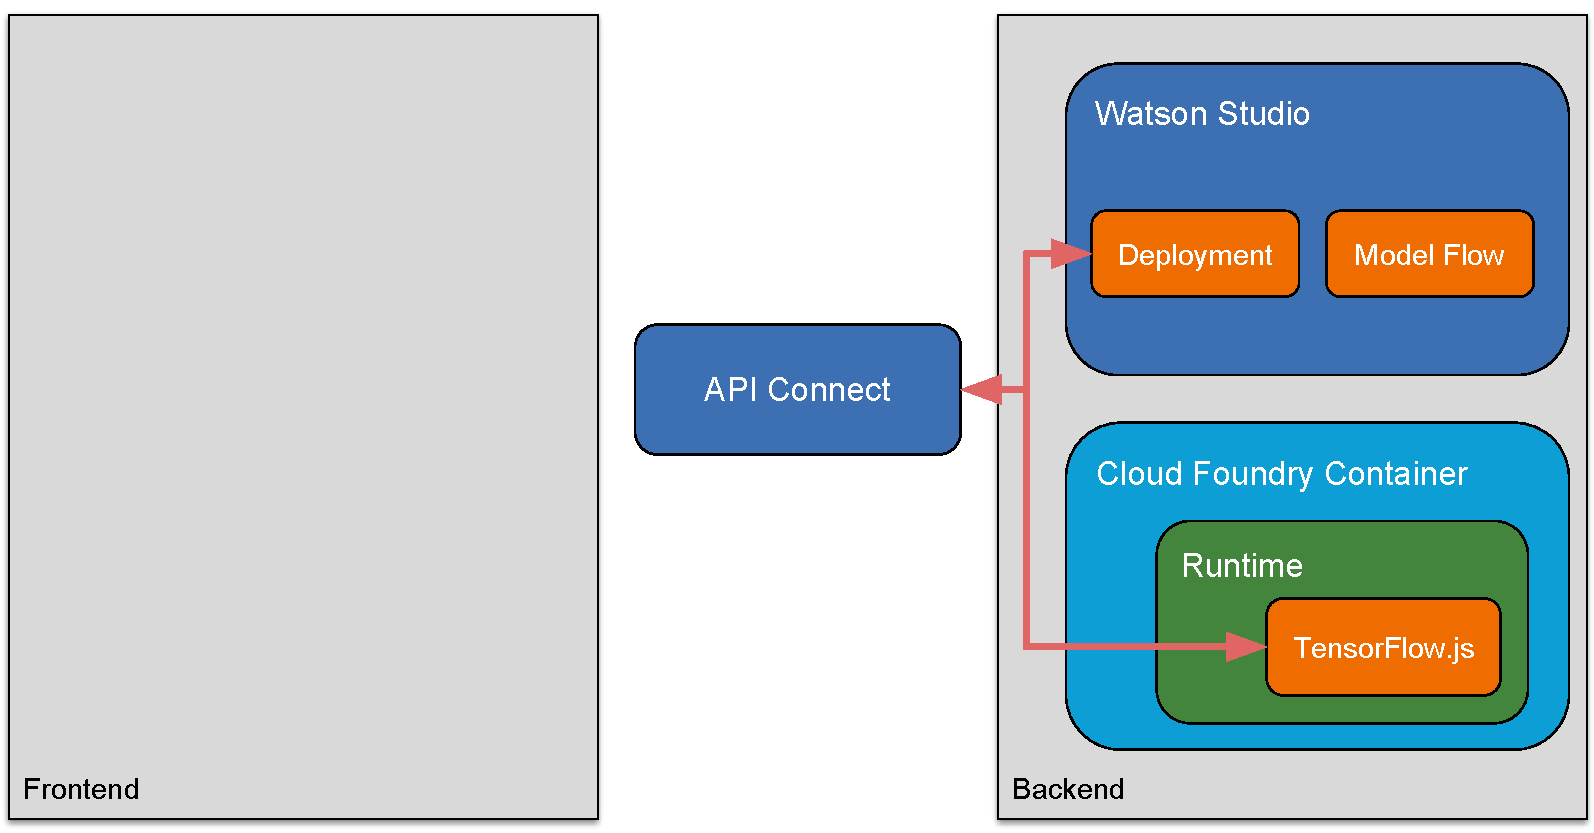
\includegraphics[width=\textwidth]{images/kapitel_3/architektur_uebersicht.pdf}
    \caption{Übersicht der Zielarchitektur}
    \label{fig:umsetzung_zielarchitektur}
\end{figure}

\subsection{Cloud}
Wie in der Vorbereitung, Kapitel~\ref{sec:analyse} auf Seite~\pageref{sec:analyse}, beschrieben, wird das neuronale Netz
in der Cloud erstellt, konfiguriert und trainiert. Wie bereits erwähnt hat dies einen enormen Geschwindigkeitsvorteil
gegenüber der offline trainierten Variante. Im Anschluss daran wird das trainierte Model heruntergeladen und mit einem
TensorFlow.js Wrapper nutzbar gemacht.

Die folgenden Kapitel beschreiben die notwendigen Schritte für die Erstellung eines neuronalen Netzes in der Cloud, das
trainierten des Models und das Einrichten eines Deployments für die REST-Schnittstelle.

\subsubsection{Daten zusammenstellen}
In einem ersten Schritt muss man die Daten, welche man später für das Training des neuronalen Netzes nutzen möchte,
sammeln und in einer Datei bündeln. Als Format eignet sich dafür eine Excel-Tabelle hervorragend, da das Anlegen der
Datensätze in Zeilen und Spalten sinnvoll ist.

Um eine Auswahl an Daten zu schaffen muss man sich darüber im klaren sein, welche Parameter existieren und welche Werte
durch das neuronale Netz vorhergesagt werden sollen. Auch ist wichtig zu wissen, welche Eingaben notwendig sind, um
überhaupt die Vorhersagen machen zu können.

In diesem Beispiel sollen Daten für das Bosch KWE Kontrollwaagensystem aufbereitet werden. Die vorhersagbaren Parameter
sind die, welche Angaben über den Pusher und über die Bandgeschwindigkeit zulassen.

Der Pusher wird durch insgesamt vier Parameter bestimmt. Die \textit{Druckluft} gibt darüber auskunft, wie stark oder
schnell der Pusher aus seiner Warteposition herausfährt. Der \textit{Impuls} gibt die Wucht an, mit der der Pusher
ausfährt.

Der Parameter \textit{Totzeit} gibt die Zeit an die gewartet wird, bis der Pusher herausfährt obwohl er schon das Signal
zum ausfahren bekommen hat. Über die \textit{Position} wird der Pusher auf der Waage positioniert. Die Angabe wird ab
dem Mittelpunkt der Wiegeeinheit gerechnet.

Für die Inputparameter, also die Parameter die später die Eingabevariablen des neuronalen Netzes sind werden alle die
genutzt, welche noch zur Verfügung stehen. Dabei handelt es sich um insgesamt 13 Stück. Sie sind in
Tabelle~\ref{tab:targets_inputs} auf Seite~\pageref{tab:targets_inputs} ersichtlich.

Alle Input-Werte sind in diesem Fall vom Kunden abhängig und desshalb problemlos Recherchierbar beziehungsweise abgelegt
und gespeichert.

In der noch leeren Excel-Tabelle muss man nun in den Spalten die Eingabeparameter aber auch die vorhersagbaren Parameter
auflisten. Jede leere Zeile wird durch ein Produkt ersetze. So listet man alle historischen Daten untereinander auf und
befüllt jede Spalte mit den entsprechenden Informationen.

Sollte man für eine Spalte keinen Wert haben, so muss die Zeile leer gelassen und es darf keine null oder sonstiges
eingetragen werden.

In Anhang~\ref{sec:scaleData} auf Seite~\pageref{sec:scaleData} sind die Beispieldaten für die Waage aufgezeigt. Die
folgenden Kapitel beziehen sich auf diesen Datensatz.

Da die Daten zusammengestellt sind, kann man sie in einem weiteren Schritt in das Watson Studio importieren um das
neuronale Netz zu trainieren.

\subsubsection{Daten importieren}
Nachdem man die Trainingsdaten zusammengestellt hat, kann man diese nun in das Watson Studio importieren. Dazu existiert
im Watson Studio Dashboard ein Menüpunkt mit dem Namen \textit{Assets} am oberen Menüband.

Dieser beinhaltet alle hochgeladenen, generierten oder gesammelten Daten, Modelle, Dashboards, Notebooks oder Flows. Die
oberste Kategorie, \textit{Data Assets}, listet alle Trainingsdaten in Form von Excel-Tabellen für die Weiterverarbeitung
auf. In diese Kategorie muss man die zuvor erstellte Tabelle hochladen.

Über den Menüpunkt \texttt{New data asset} kann man die erstellte Datei hochladen. Ein Klick auf diesen Menüpunkt öffnet
einen seitlichen Arbeitsbereich. Der Nutzer kann über den Menüpunkt \texttt{Browse} die Dateiauswahl des Betriebssystems
öffnen und seine Datei auswählen. Bei der Auswahl handelt es sich um die im vorangegangenen Kapitel erstellte Datei mit
Trainingsdaten.

Alternativ kann man die Datei auch in das fabrlich hervorgehobene Feld schieben. Der Upload der Datei startet damit
sofort.

Nach wenigen Sekunden ist die Datei hochgeladen und wird im Bereich \textit{Data assets} angezeigt. Damit ist der
Uploadvorgang erfolgreich abgeschlossen und die Datei kann im nächsten Schritt umgewandelt werden.

\subsubsection{Daten umwandeln}
Da die erstellte Datei mit den Trainigsdaten nun in Watson Studio bereitsteht, ist die Umwandlung in eine CSV-Datei
möglich. Dieser Schritt ist zwingend notwendig, damit die Datei später als Eingabeparameter für das neuronale Netz
dienen kann. Ein anderes Format wird als Eingabe zur Zeit nicht unterstützt.

In Watson Studio liegt mit den \textit{Data flows} ein einfaches Werkzeug bereit, um Dateien in das benötigte CSV-Format
zu überführen. Dazu kann der Nutzer in der Kategorie Data Flows über \texttt{New data flow} ein neuer Flow anlegen.

Im folgenden öffnet sich der Wizzard zum Erstellen des Flows. Der Nutzer muss im linken Bereich die umzuwandelnde Datei
auswählen. Dabei handelt es sich um die hochgeladene Datei. Über die Schaltfläche \texttt{Add} kann man die Auswahl
übernehmen.

Nun ist der Inhalt der Datei im mittleren Bereich des Displays sichtbar. Bei dieser Ansicht ist darauf zu achten, dass
die Interpretation der Werte der einzelnen Spalten als Dezimal-Zahl erfolgt. Diese Information steht unterhalb der
einzelnen Spaltenüberschriften. Sollte diese Einstellung nicht voreingestellt sein, muss man diese manuell abändern.

Dazu klickt man in der entsprechenden Spalte oben, rechts neben dem Spaltenname, auf die drei Punkte (Einstellungen) und
selektiert den Eintrag \texttt{Convert Column}. Im Untermenü muss man dann den Wert \texttt{Decimal} bestätigen. Nun
werden die Zahlen in der Spalte auch korrekt als Dezimal-Zahl interpretiert.

Da es sich bei allen Zahlen nun um Dezimal-Zahlen handelt, kann man über die Schaltfläche \texttt{Run data flow} die
Konvertierung starten. Bevor die Konvertierung jedoch startet, zeigt das System eine Übersicht über die einzelnen
Schritte, die dazu benötigt werden, an.

Hier werden zum Beispiel etwaige Konvertierungen zu Dezimal-Zahlen angezeigt oder sonstige Operationen dargestellt. Da
es sich hierbei lediglich um Informationen handelt, kann der Nutzer die Seite bestätigen und der Flow startet.

Nach wenigen Minuten sollte im Watson Studio im Bereich Assets, in der Kategorie Data Assets, die neue Datei zur
Verfügung stehen. Dabei trägt die Datei die Dateiendung \textit{.csv}. Die Konvertierung der Datei ist somit
abgeschlossen und man kann sie für das neuronale Netz verwenden.

\subsubsection{Modeler Flow}
\label{subsub:modeler_flow}
Nach erfolgreicher Konvertierung der Trainingsdaten kann man diese für das neuronale Netz nutzen. Für die Erstellung
des neuronalen Netzes und den damit verbundenen Parameterübergaben für die Vorhersage ist der \texttt{Modeler Flow} am
Besten geeignet.

Über die Schaltfläche \texttt{New Flow} im Bereich Assets erstellt man diesen und richtet ihn ein. Nachdem man einen Namen
und eine optionale Beschreibung für den Flow eingegeben hat, muss man die Auswahl \textit{Modeler Flow} und
\textit{IBM SPSS Modeler} auswählen. Dabei handelt es sich um den Standard-Flow von Watson Studio.

Der Nutzer bestätigt die Eingabe über die Schaltfläche \texttt{Create} und nach kurzer Zeit ist der Flow erstellt und es
erscheint ein leerer Arbeitsbereich im Browser.

Der Menüpunkt \texttt{Palette} zeigt einen linken Arbeitsbereich mit allen aktuell verfügbaren Modulen, gruppiert an. In
diesem muss man den Baustein \textit{Data asset} in der Gruppe \textit{Import} auswählen.

Dieser Baustein ermöglicht den Import der konvertierten Trainingsdaten für das neuronale Netz. Über Drag \& Drop kann der
Nutzer den Baustein in den noch leeren Arbeitsbereich platzieren.

Um den Baustein zu konfigurieren Klickt der Entwickler doppelt auf den Baustein. Daraufhin öffnet sich ein rechter,
seitlicher Arbeitsbereich. In diesem kann er über die Schaltfläche \texttt{Change Data Asset} die Datei auswählen, welche
die Trainingsdatensätze enthält.

In dieser Liste steht lediglich die vorher erstellte CSV-Datei zur Verfügung, da bisher lediglich CSV-Dateien als
Eingabeparameter genutzt werden können. Über \texttt{Save} wird die Einstellung gespeichert und der Baustein ist fertig
konfiguriert.

Im nächsten Schritt erfolgt die Konfiguration des neuronalen Netzes. Dazu existiert in der Kategorie \textit{Modeling}
das Modul \textit{Neural Net}. Das stellt für den Anwendungsfall die beste Alternative dar, da es sich hierbei um ein
allgemeines neuronales Netz handelt. Dies kann allerdings sehr tief konfiguriert werden.

Genau wie das Import-Modul kann man dieses mit der Maus in einen freien Bereich des Arbeitsbereiches platzieren. Somit
ist das Modul Teil des Prozesses und der Entwickler kann es konfigurieren.

Damit das neuronale Netz die importierten Datensätze nutzen kann, wird eine Verbindung zwischen dem \textit{Import-Modul}
und dem \textit{Neural-Net-Modul} aufgebaut. Mit einen Klick auf den Ausgang des Import-Moduls startet man eine
Verbindungslinie.

Mit einem anschließenden Klick auf den Eingang des Neural-Net-Modul kann man die Verbindung fertig aufbauen. Die Verbindung
wird nun über eine durchgezogene Linie zwischen den beiden Modulen visualisiert.

Bei einer Verbindung wird der Output eines Modules an das mit einer visualisierten Linie verbundenen Modul weitergegeben.
Dieses Folgemodul kann die Werte dann als Eingabevariablen nutzen. Einen Ausgang kann man mit mehreren Eingängen
verbinden. Dabei stehen dann allen weiteren Modulen die gleichen Werte zur Verfügung.

Die Konfiguration des Neural-Net-Moduls erfolgt durch einen doppelten Klick auf dieses. Damit man die
\textit{Targets} und die \textit{Inputs} selbst definieren kann, muss man den Hacken bei \enquote{Use custom field roles}
setzen. Andernfalls versucht Watson selbst die Inputs und die Outputs zu definieren. Meist sind diese Einstellungen dann
aber falsch.

Die Tabelle~\ref{tab:targets_inputs} auf Seite~\pageref{tab:targets_inputs} zeigt die auszuwählenden Tabellenspalten für
die jeweilige Kategorie. Die Targets beschreiben die Variablen, welche durch den Watson Service Vorhergesagt werden
sollen. Die Inputs definieren die Größen, durch welche eine Vorhersage überhaupt möglich ist.

Dem resultierenden, trainierten Model werden zu einem späteren Zeitpunkt die Inputs übergeben und die Targets kommen als
vorhergesagte Rückgabeparameter zurück.

\begin{table}[h]
    \centering
    \begin{tabular}{|c|c|}
        \hline
        \textbf{Targets} & \textbf{Inputs}\\
        \hline
        \hline
        Leistung & Einlaufbandlänge\\
        \hline
        Druckluft & Wägebandlänge\\
        \hline
        Impuls & Auslaufbandlänge\\
        \hline
        Totzeit & Einlaufbandbreite\\
        \hline
        Position & Wägebandbreite\\
        \hline
        & Auslaufbandbreite\\
        \hline
        & Einlaufbandrolle\\
        \hline
        & Wägebandrolle\\
        \hline
        & Auslaufbandrolle\\
        \hline
        & Produktbreite\\
        \hline
        & Produktlänge\\
        \hline
        & Produkthöhe\\
        \hline
        & Packungsgewicht\\
        \hline
    \end{tabular}
    \caption{Variablen für die Targets und die Inputs}
    \label{tab:targets_inputs}
\end{table}

Mit dieser Konfiguration werden 13 Parameter als Eingabevariablen genutzt und fünf Parameter durch das neuronale Netz
vorhergesagt.

Vier der vorhergesagten Parameter (Druckluft, Impuls, Totzeit und Position) beziehen sich auf den \textit{Pusher} und
der Parameter \textit{Leistung} gibt die tatsächliche Bandgeschwindigkeit an, mit der das Band in der Maschine laufen
soll.

Alle anderen Einstellungen des neuronalen Netzes werden im ersten Schritt auf den Standardeinstellungen belassen. Zu
einem späteren Zeitpunkt, wenn sich Testdaten ändern oder Parameter angepasst werden müssen, kann man mit den weiteren
Einstellungen das neuronale Netz anpassen und gegebenenfalls optimieren.

Der Flow für das neuronale Netz ist somit fertiggestellt. Mit einem Klick auf \texttt{Run} startet das Training des
neuronalen Netzes.

Nach dem erfolgreichem Training des neuronalen Netzes erscheint das trainierte Model unterhalb des neuronalen Netzes im
aktuellen Arbeitsbereich. Eine gestrichelte Linie zwischen dem neuronalen Netz und dem trainierten Model zeigt die
Abhängigkeit der beiden Module an.

Für die Weiterverarbeitung und ein späteres Deployment des trainierten Models muss man dieses mit einem Export-Modul
verbinden. Der Export erfolgt über das Modul \textit{Table}.

Das Table-Modul befindet sich in der Kategorie \textit{Outputs} und wird, genau wie alle andere Module, frei auf dem
Arbeitsbereich platziert. Eine Verbindung zwischen dem trainierten Model und der Table ermöglicht den Datenaustausch.
Für die Table ist keine weitere Konfiguration notwendig.

Ein Rechtsklick auf das Table-Modul öffnet das Kontextmenü des Moduls. Darüber lässt sich der Punkt
\enquote{Save branch as a model} anklicken. Dieser ermöglicht es, das trainierte Model zu exportieren.

In dem sich öffnenden Fenster muss man den Namen und eine optinale Beschreibung für das neue Model definieren. Mit einem
Klick auf den Button \texttt{Save} wird das Model gespeichert und es erscheint im Watson Studio Dashboard.

In der Abbildung~\ref{fig:umsetzung_model_flow} auf Seite~\pageref{fig:umsetzung_model_flow} ist der vollständige Aufbau
des Model Flows dargestellt mit seinem trainierten Model und der Tabellen-Exportierung.

\begin{figure}[h]
    \centering
    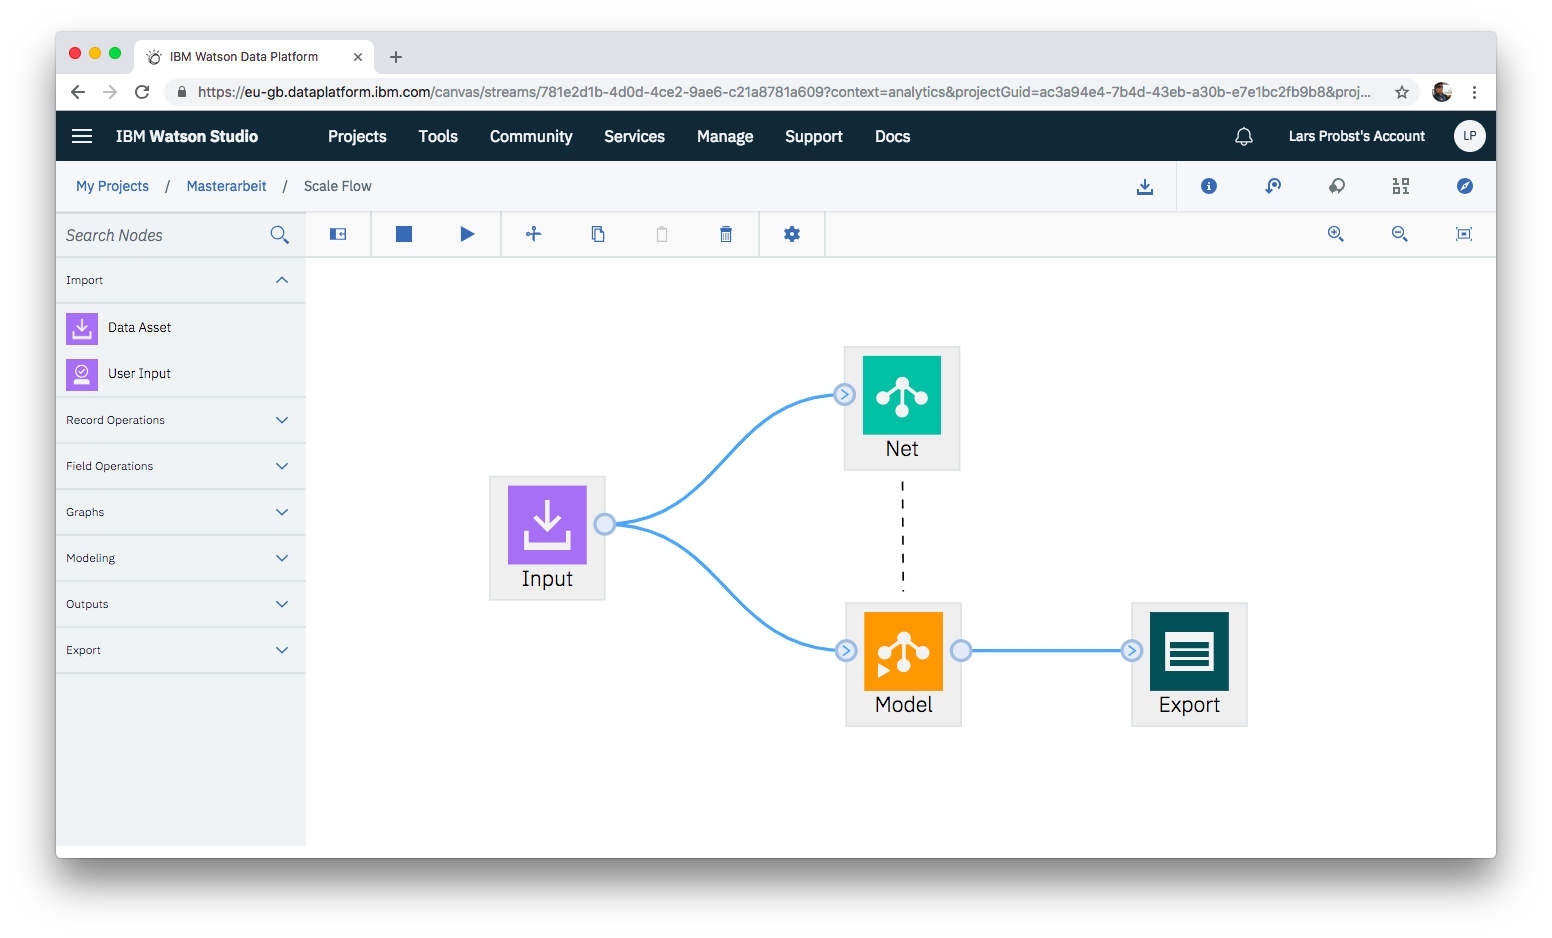
\includegraphics[width=\textwidth]{images/kapitel_3/umsetzung_model_flow.png}
    \caption{Vollständiger Model Flow}
    \label{fig:umsetzung_model_flow}
\end{figure}

\subsubsection{Informationen zum Model}
Über einen weiteren Rechtsklick auf das trainierte Model kann man über den Menüpunkt \texttt{View Model} auf eine
detaillierte Übersicht des Models gelangen. Hier finden sich zahlreiche Informationen, die unter anderem Aufschluss
über die Genauigkeit des Models geben.

Die erste Information, welche man als Benutzer über das Model zu sehen bekommt, ist in
Abbildung~\ref{fig:umsetzung_model_evaluation} auf Seite~\pageref{fig:umsetzung_model_evaluation} zu sehen \textendash{}
die \texttt{Evaluation}.

\begin{figure}[h]
    \centering
    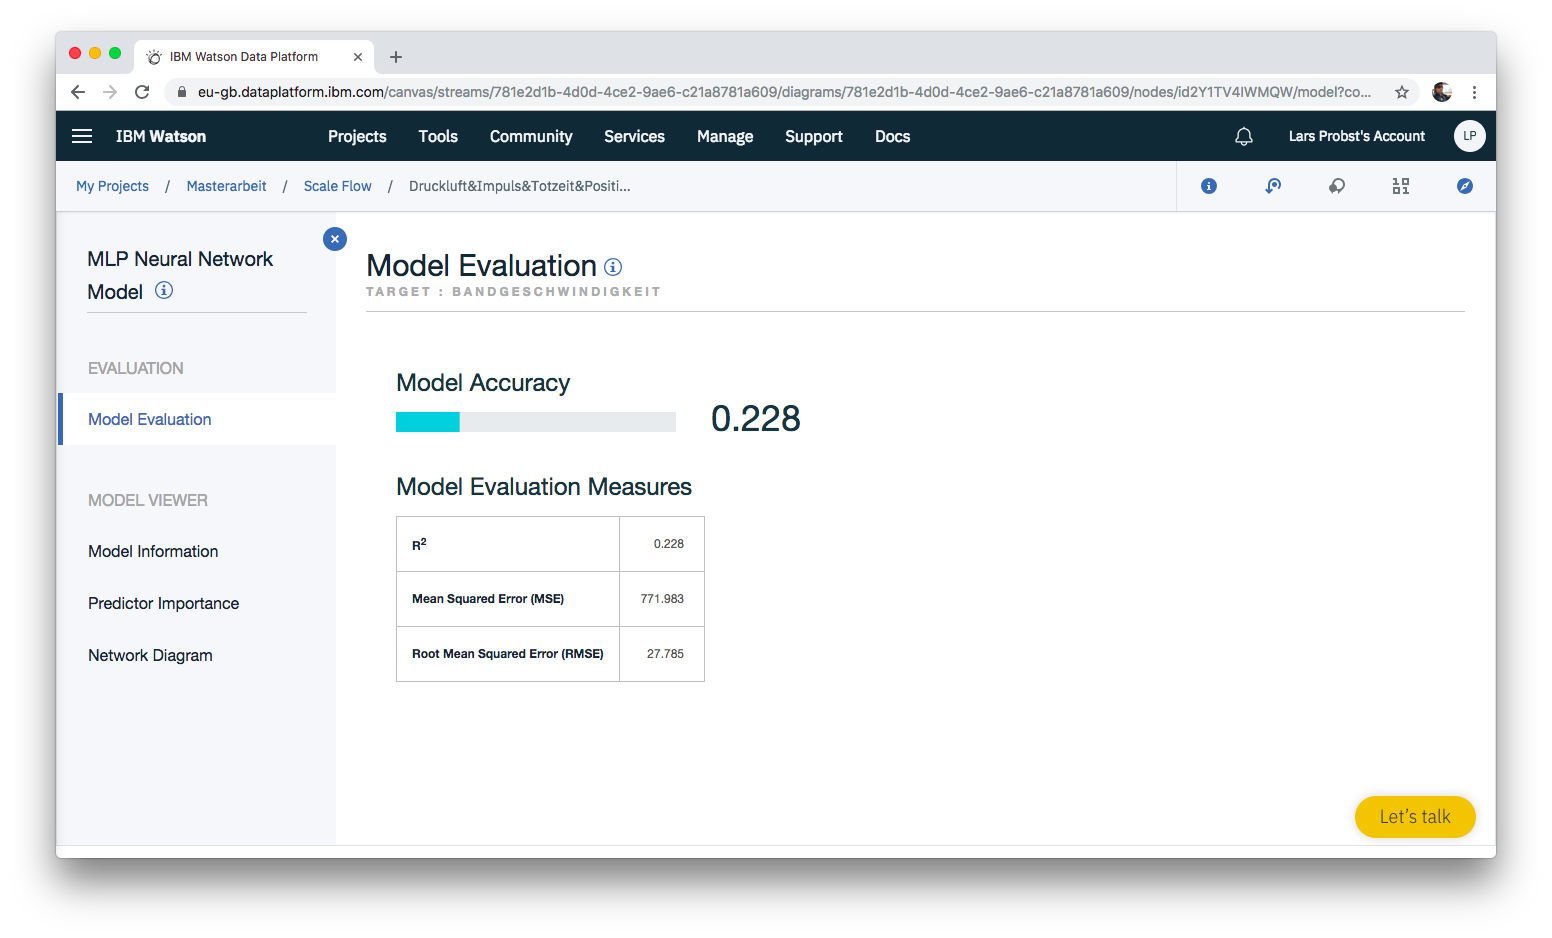
\includegraphics[width=\textwidth]{images/kapitel_3/model_evaluation.png}
    \caption{Evaluation des trainierten Models}
    \label{fig:umsetzung_model_evaluation}
\end{figure}

Die große Zahl gibt die tatsächliche Genauigkeit des Models (englisch Model Accuracy) an. Mit 100 multipliziert, erhält
man die prozentuale Angabe der Genauigkeit. Wenn man mit dem Mauszeiger über die Zahl fährt, erhält man eine genauere
Angabe mit Nachkommastellen.

Die Genauigkeit berechnet sich durch ein Testdatenset, welches dem Trainingsdatenset automatisch entnommen wird. Dabei
kann beim trainieren des Models angegeben werden, um wie viele Datenset es sich handeln soll.

Nachdem das Model fertig trainiert ist, wird es mit den zur Verfügung stehenden Testdaten gefüttert. Im Anschluss werden
die vorhergesagten Werte mit denen im Testdatenset verglichen. Je größer die Abweichung ist, desto geringer ist die
Genauigkeit des trainierten Models.

Im Weiteren finden sich Bewertungskriterien für das trainierte Model (englisch Model Evaluation Measures). Diese geben
Aufschluss darüber, wie gut das Model ist. In der ersten Zeile wird zum Beispiel $\mathbf{R^2}$ ausgegeben.  Dabei
handelt es sich um den Determinationskoeffizient. Dieser ist eine wichtige Kennzahl zur formalen Beurteilung der
Regression. Weitere Informationen sind auf der Wikipedia-Seite\footnote{https://de.wikipedia.org/wiki/Bestimmtheitsmaß}
ersichtlich.

Der nächste Wert entspricht der \enquote{Mittleren quadratische Abweichung} (englisch Mean Squared Error). Dies ist der
Durchschnitt der quadrierten Fehler. Als Fehler ist die Differenz der vorhergesagten Werte und der tatsächlichen Werte
definiert.

Der letzte Wert gibt das \enquote{Mittleres Abweichungsquadrat} (englisch Root Mean Squared Error) an. Dieser Wert ist
ein Maß für die Unterschiede zwischen Werten, die von einem Modell vorhergesagt werden, und den tatsächlich beobachteten
Werten.

In der nächsten Kategorie, Model Viewer, sind Informationen zu den einzelnen Werten des neuronalen Netzes angegeben.
Im ersten Menüpunkt, Model Information, stehen alle generellen Informationen.

Mit einem Klick auf den Menüpunkt gelangt man in eine Ansicht wie in Abbildung~\ref{fig:umsetzung_model_information}
auf Seite~\pageref{fig:umsetzung_model_information} zu sehen.

\begin{figure}[h]
    \centering
    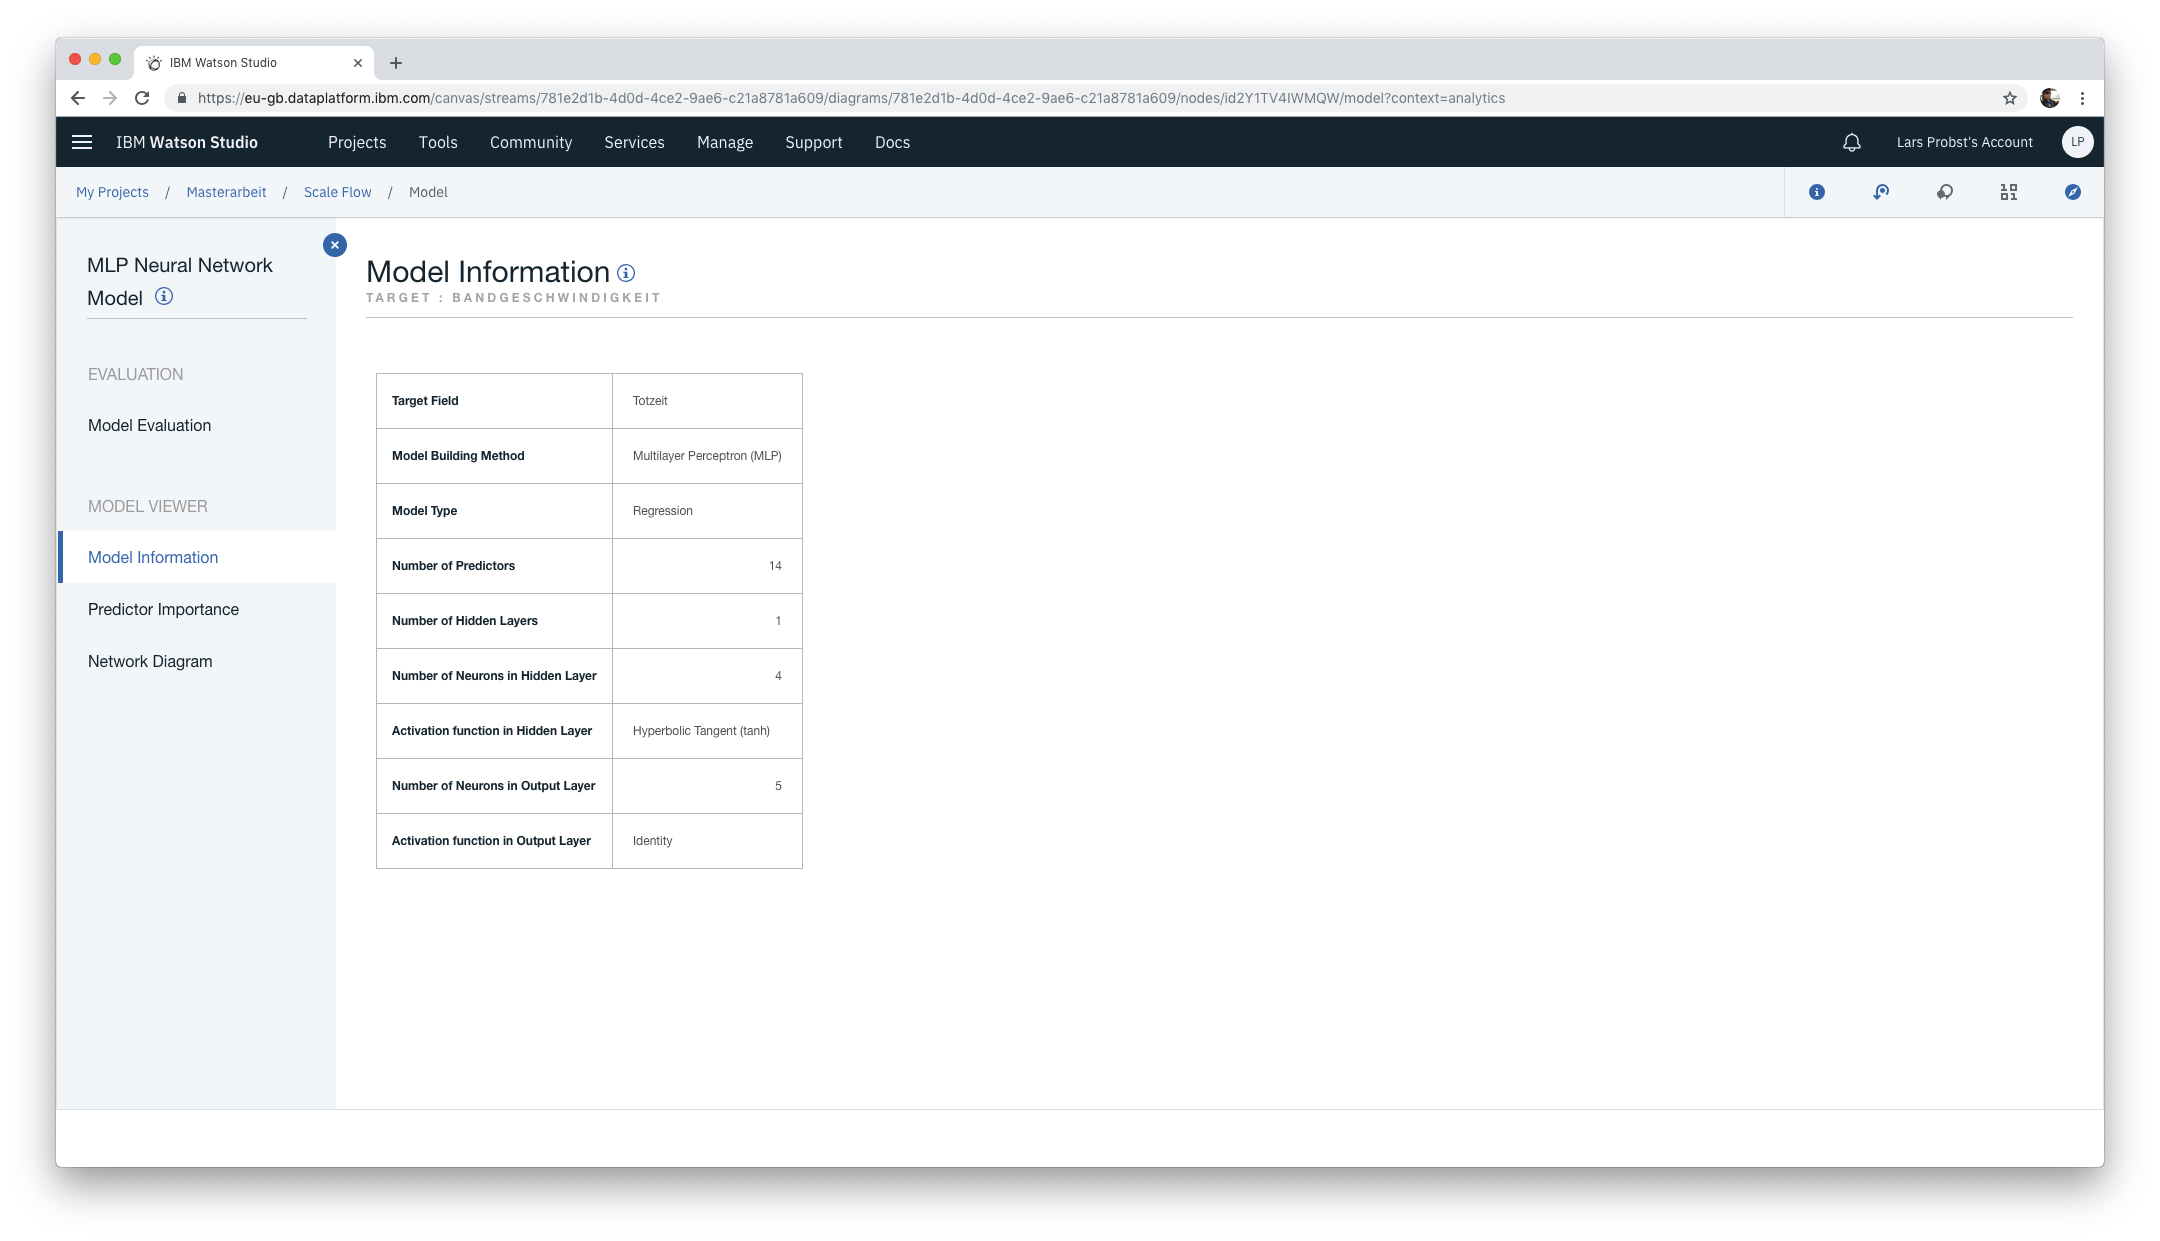
\includegraphics[width=\textwidth]{images/kapitel_3/model_information.png}
    \caption{Informtionen zum trinierten Model}
    \label{fig:umsetzung_model_information}
\end{figure}

Hier findet man Informationen darüber, wie das trainierte Model aufgebaut ist oder um welche Art Model es sich handelt.
Auch die Hiden Layers, die im neuronalen Netz eingerichtet sind, werden hier angegeben.

Weiter ist hier zu finden, mit wie vielen Inputparametern (englisch Number of Predictors) das Netz trainiert ist und wie
viele Ausgabewerte (englisch Number of Neurons in Output Layer) das Netz vorhersagen kann.

Im Menüpunkt \texttt{Predictor Importance} sind alle Input-Parameter aufgelistet. Ein Balken unterhalb jedes Parameters
gibt an, wie wichtig dieser für das neuronale Netz ist. In Abbildung~\ref{fig:umsetzung_model_predictor} auf
Seite~\pageref{fig:umsetzung_model_predictor} ist dies beispielhaft aufgezeigt.

\begin{figure}[h]
    \centering
    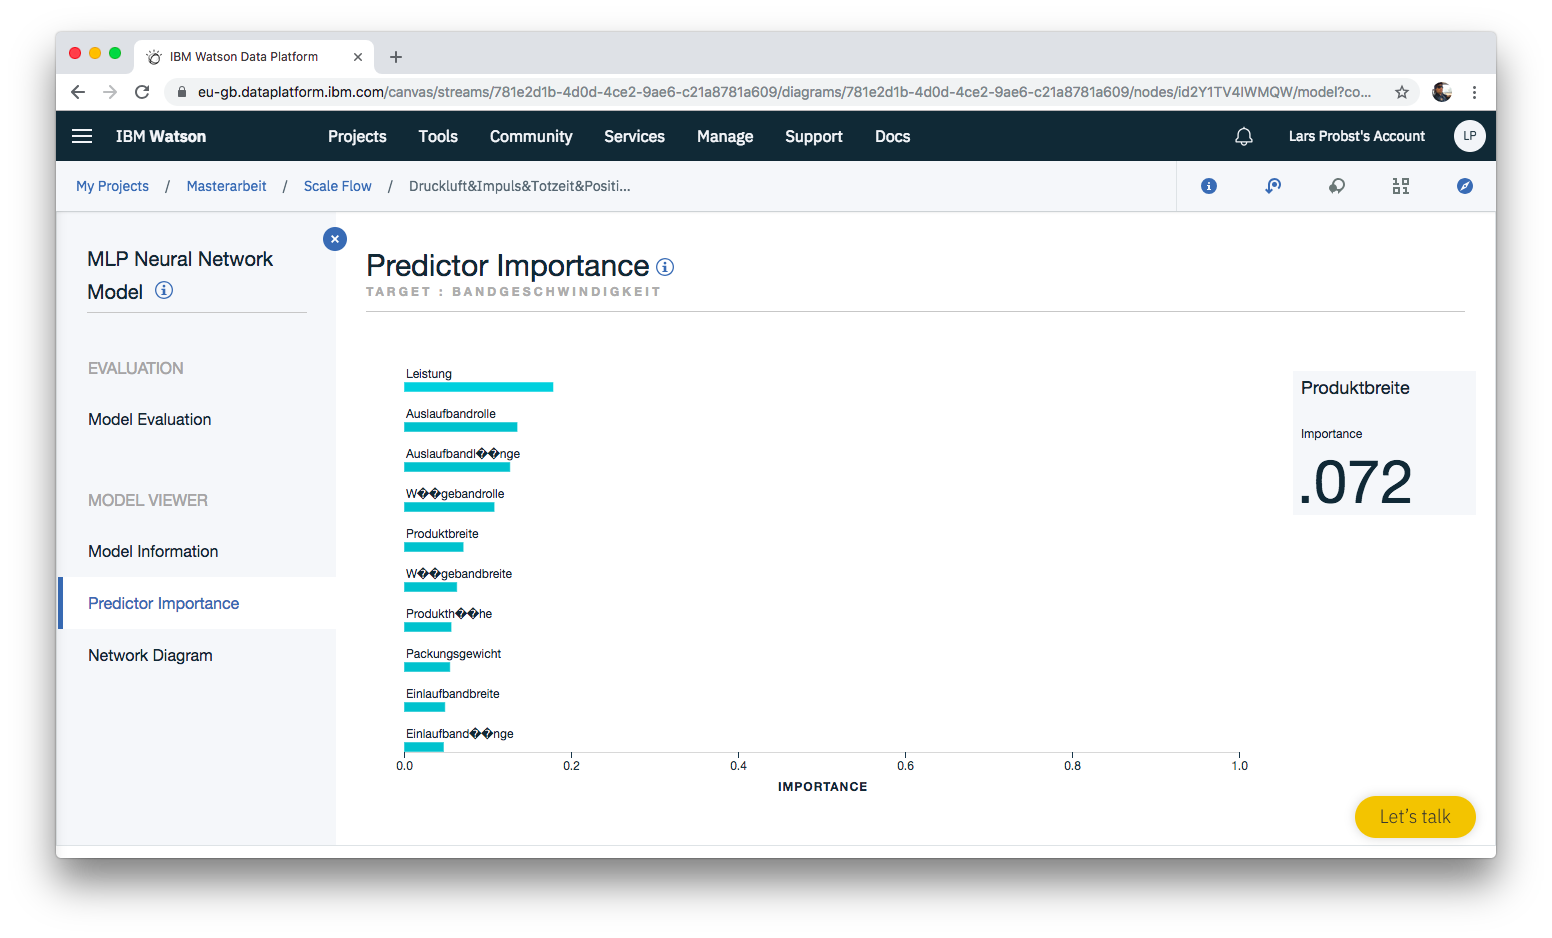
\includegraphics[width=\textwidth]{images/kapitel_3/model_predictor.png}
    \caption{Wichtigkeit der einzelnen Eingabeparameter}
    \label{fig:umsetzung_model_predictor}
\end{figure}

Beim Überfahren eines jeden Parameters wird der prozentuale Wert am rechten Rand dargestellt. Je wichtiger ein Parameter
ist, desto mehr Einfluss hat dieser auf die vorhergesagten Ausgabewerte.

Parameter mit der geringsten Gewichtung spielen für das Ergebnis keine große Rolle und könnten bei einer Optimierung des
neuronalen Netzes weggelassen werden.

Der letzte Menüpunkt, mit der Aufschrift \texttt{Network Diagram}, zeigt das neuronale Netz, wie es beim Traning aufgebaut
wurde. Dabei sind auf der linken Seite die Parameter zur Eingabe aufgelistet.

Auf der rechten Seite erscheinen die Ausgabeparameter. Dazwischen werden die \textit{Hidden Layers} dargestellt und wie
diese mit der Eingangs- und Ausgangsseite verbunden sind. Die Abbildung~\ref{fig:umsetzung_model_network_diagram}
auf~\pageref{fig:umsetzung_model_network_diagram} visualisiert das vorangegangene, trainierte Model.

\begin{figure}[h]
    \centering
    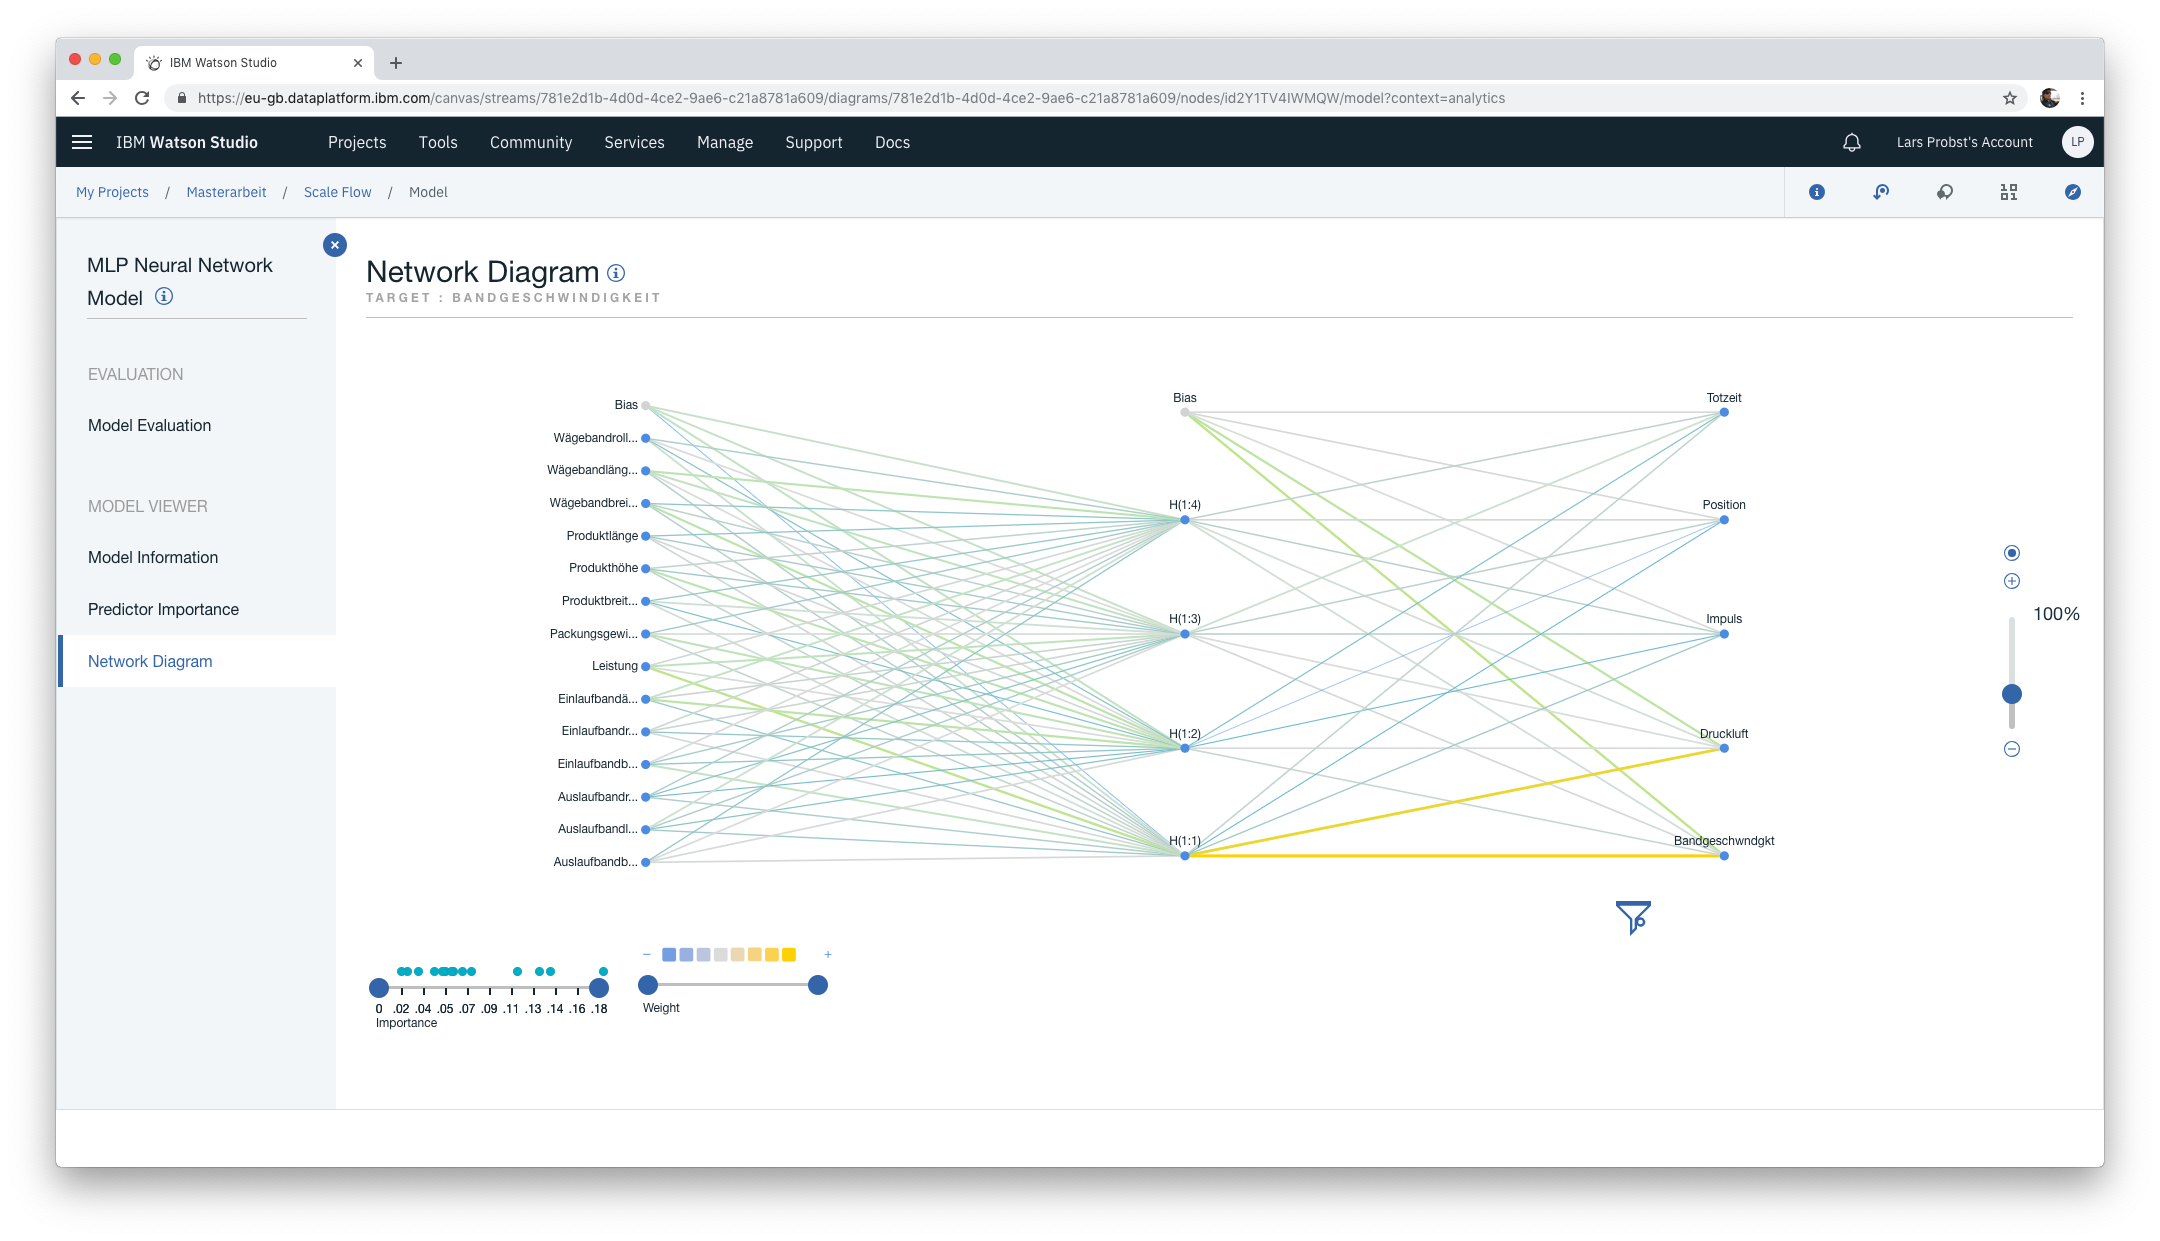
\includegraphics[width=\textwidth]{images/kapitel_3/model_network_diagram.png}
    \caption{Übersicht des trainierten Netzes}
    \label{fig:umsetzung_model_network_diagram}
\end{figure}

Die Ansicht kann man über den Slider am rechten Bildschirmrand vergrößern oder verkleinern. Über die Legende am unteren
Rand, kann man die einzelnen Verbindungen filtern.

So ist es zum Beispiel möglich, dass man sich alle Verbindungen mit hoher Priorität anzeigen lässt. Damit hat der
Entwickler eine Visualisierung, wie die wichtigsten Eingabeparameter für die entsprechenden Ausgaben sorgt.

Auch kann man sich so anzeigen lassen, wie einzelne Werte auf der Eingabeseite einen direkten Einfluss auf einen
Ausgabewert haben. Im Beispiel der Abbildung hat der Parameter \textit{Leistung} einen direkten und sehr großen
Einfluss auf den Ausgabewert \textit{Bandgeschwindigkeit}.

Bei weiterer Betrachtung ist diese Zusammenhang einläuchtend. Wenn mehr Produkte über die Wiegeeinheit laufen sollen (es
soll die Leistung erhöht werden), muss das Band mit höherer Geschwindigkeit (Bandgeschwindigkeit) laufen um die Produkte
zu transportieren.

Desweiteren hat die Leistung einen direkten Einfluss auf den Parameter \textit{Druckluft}. Dieser gibt indirekt die
Geschwindigkeit an, mit welcher der Pusher ausschlagen soll um ein Produkt vom Band zu hauen.

Auch dieser Zusammenhang ergibt Sinn, da eine höhere Bandgeschwindigkeit auch ein schnelleren Pusher voraussetzt, um ein
Produkt auch vom Band stoßen zu können. Das Timing ist an dieser Stelle von großer Bedeutung.

\subsubsection{Deployment erstellen}
Das in einem vorangegangenen Kapitel erstellte und trainierte Model kann man im Weiteren durch ein Deployment über eine
REST-Schnittstelle in einem Web-Dienst verfügbar machen.

Dazu ist es erforderlich, das Model in einen \texttt{Web service} zu installieren. Die spätere Wartung und Verwaltung
des Deployments wird dabei automatisch von der IBM Cloud übernommen.

Für die Erstellung des Web Services muss man im Watson Dashboard das zuvor erstellte Model auswählen. Das folgende
Fenster zeigt mehrere Informationen zu diesem an. Unter anderem ist sichtbar, welche Eingabe- und Ausgabeparameter für
das Model wichtig sind.

Der Reiter \texttt{Evaluation} zeigt vorangegangene Auswertungen des Models an. Über den Menüpunkt \texttt{Lineage}
werden Verknüpfungen und Abstammungen des Models angezeigt.

Für das Deployment ist der Reiter \texttt{Deployments} wichtig. Dieser verwaltet alle Deployments des einen Moduls. Das
Löschen von älteren Deployments oder das Erstellen von Neuen ist hier möglich. Die Schaltfläche \texttt{Add Deployment}
öffnet eine Konfigurationsseite zum Erstellen eines neuen Deployments.

Ein Model kann über mehrere Deployments verfügbar gemacht werden. So ist es möglich, die Last eines Web-Services zu
reduzieren bzw. auf mehrere zu verteilen. Um die Last zu verteilen bedarf es eines Load-Balancers.

Als Type für das Deployment muss man \textit{Web Service} auswählen. Der Name des Deployments ist das einzige Pflichtfeld
und muss befüllt sein. Anschließend kann man das Deployment über \texttt{Save} speichern und starten. Dieser Vorgang kann
wenige Minuten dauern.

Direkt nachdem das Deployment fertiggestellt ist, wird in der Spalte \textit{Status} der Wert \texttt{DEPLOY\_SUCCESS}
angezeigt. Die Informationsseite des Deployments kann man über einen Klick auf den Namen öffnen.

Das Deployment ist somit erfolgreich erstellt und kann im Weiteren getestet und genutzt werden.

\subsubsection{Deployment testen}
Ein online Test des eingerichteten Deployments ist über das Watson Studio Dashboard möglich. Dies hat den Vorteil, dass
man das Deployment direkt testen und bei Fehlveralten neu trainiert kann. Auch benötigt man keine externe Software um
das Model zu testen.

Auf der Deploymentseite des gespeicherten Models genügt ein Klick auf den Namen um die Deploymentinformationen anzuzeigen.
Hier steht neben diversen Informationen auch der Menüpunkt \texttt{Test} zur Verfügung. Mit diesem öffnet sich eine
zweispaltige Ansicht.

In der linken Spalte befinden sich die Eingabefelder für das trainierte Model (die Inputs). Nachdem man alle Felder mit
Testwerten gefüllt hat, kann man über die Schaltfläche \texttt{Predict} eine Vorhersage starten.

Nach wenigen Sekunden erscheint auf der rechten Seite ein großes JSON-Objekt, welches den Rückgabewert des Web Services
enthält. Das erste Array, \textit{fields}, listet alle an den Web-Service gesendeten Felder auf (die Inputs).

Das zweite Array, \textit{values}, listet alle an den Web-Service gesendeten, wie auch die vorhergesagten Werte (die
Inputs und die Targets) auf. Die letzten fünf Werte des Arrays entsprechen den Vorhersagen des trainierten Models (also
die Targets). Sie entsprechen den definierten Targets.

In Abbildung~\ref{fig:umsetzung_deployment_test} auf Seite~\pageref{fig:umsetzung_deployment_test} ist ein Beispiel für
den online Aufruf des trainierten Models sichtbar.

Sollte das Array \textit{values} kleiner sein, als das Array \textit{fields}, war das trainieren des Models nicht
erfolgreich und muss wiederholt werden. Das Model kennt damit keine Targets die es vorhersagen könnte.

Unter dem Menüpunkt \texttt{Implementation} sind wichtige Informationen und erforderliche Schritte aufgezeigt, damit
man die erstellte Schnittstelle in ein eigene Programm integriert kann. Dabei wird auf verschiedene Programmiersprachen
und Architekturen eingegangenund.

\begin{figure}[h]
    \centering
    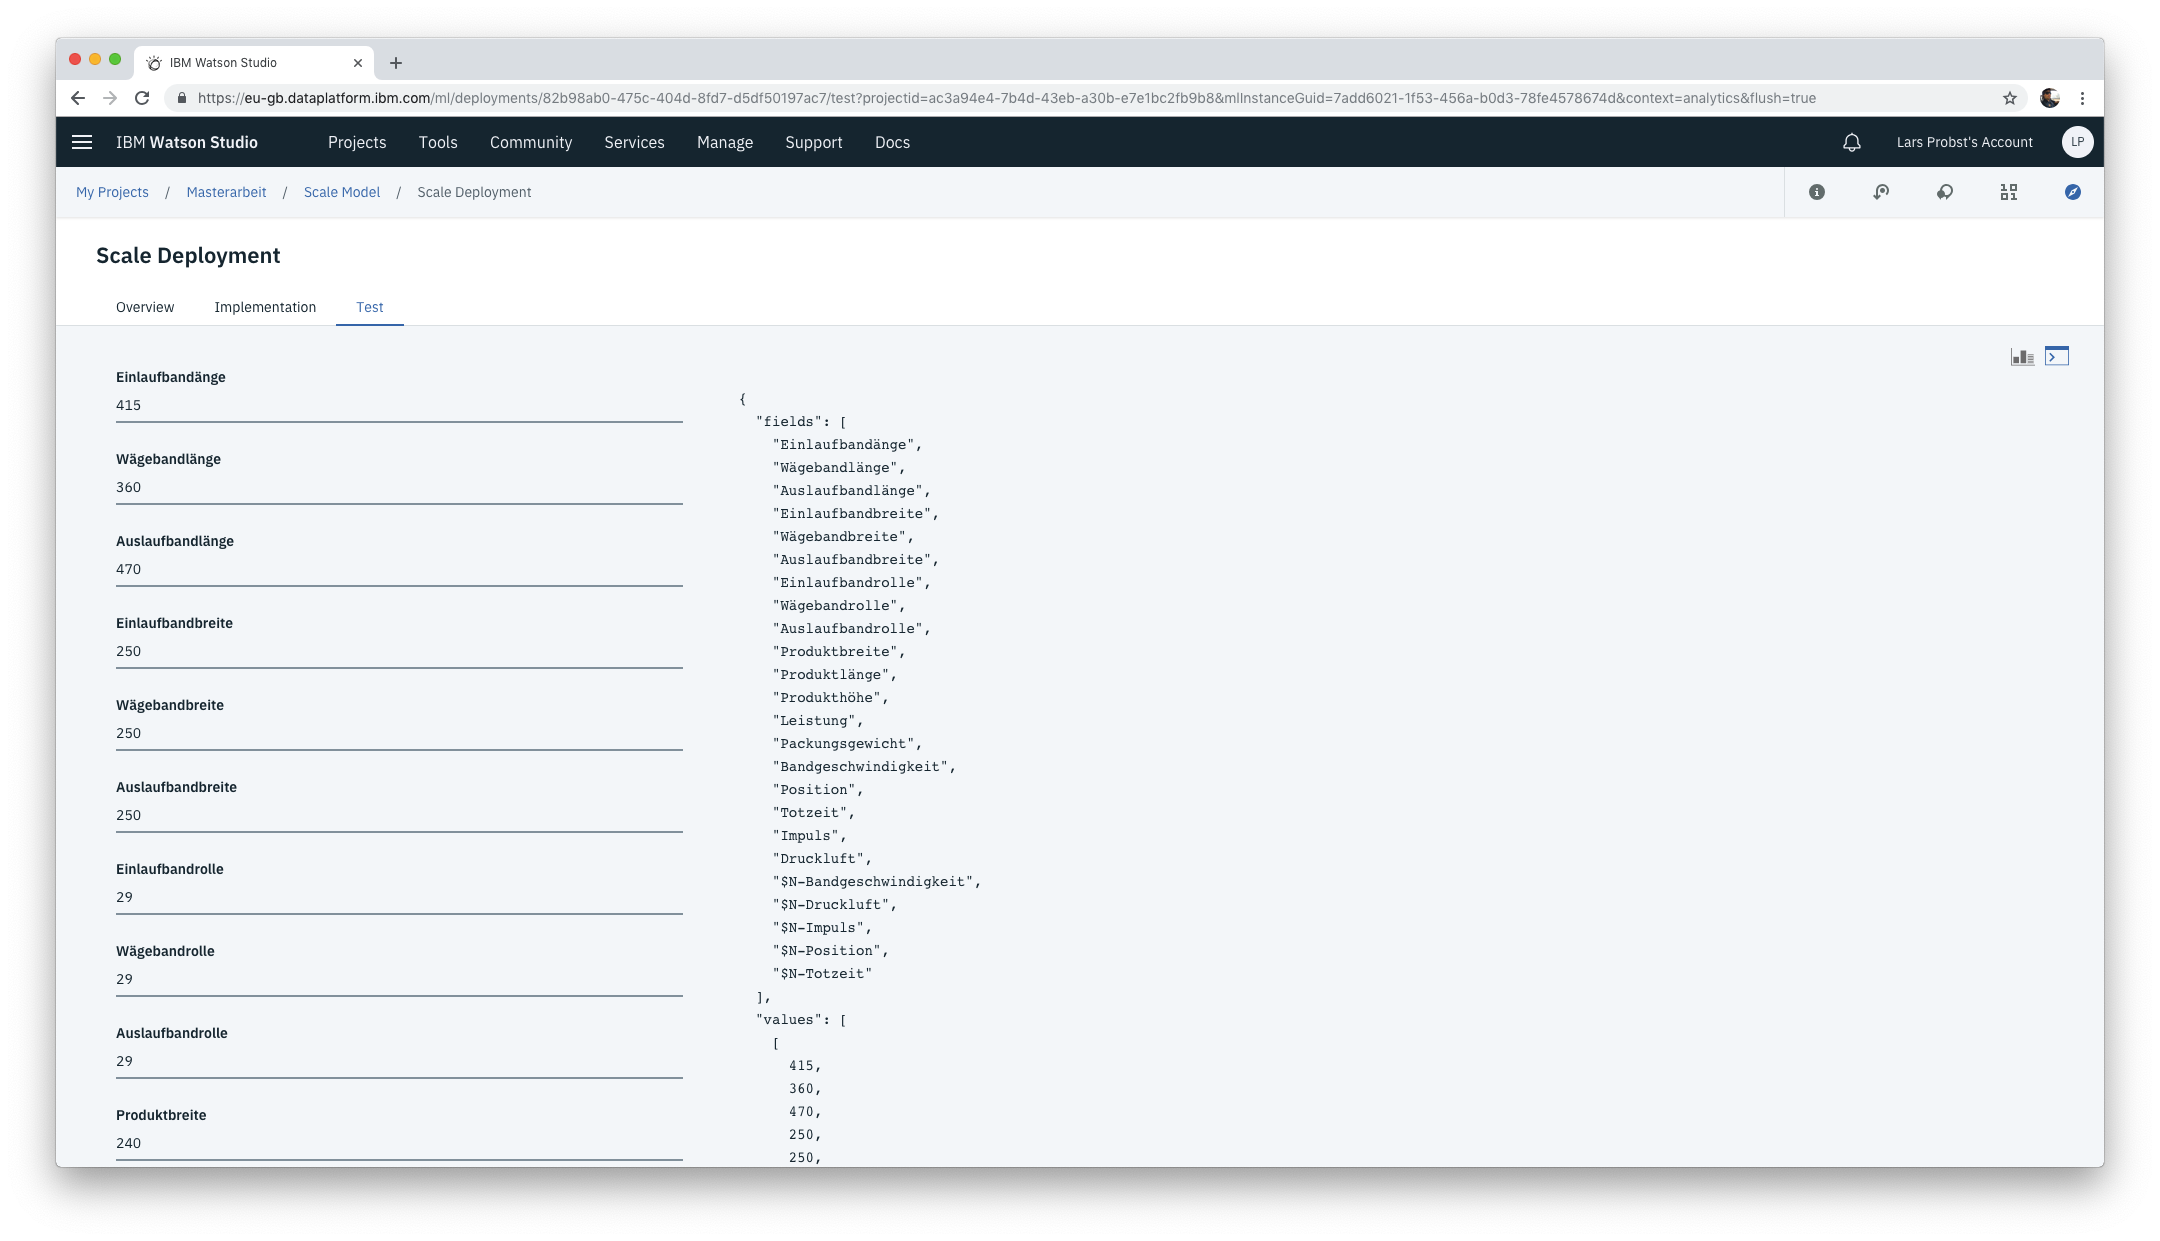
\includegraphics[width=\textwidth]{images/kapitel_3/deployment_test.png}
    \caption{Online Test des trainierten Models}
    \label{fig:umsetzung_deployment_test}
\end{figure}

\subsubsection{Aufruf mit Postman}
\label{subsec:Aufruf mit Postman}
Im Weiteren soll das erstellte Model, welches im vorherigen Kapitel als Deployment in einen Web-Service zur Verfügung
gestellt wurde, mit Postman\footnote{https://www.getpostman.com} getestet werden.

So ist sichergestellt, dass man das Model auch von extern, nicht nur über das Watson Studio Dashboard, aufrufen kann.
Dies ist für die spätere Entwicklung des Frontends und die Einrichtung des API Connect Services wichtig. Außerdem ist
so eine Überprüfung der Übergabeparameter, sowie der Rückgabewerte an die Schnittstelle möglich.

Jeder Request an den Web-Service des trainierte Models benötigt einen \textit{Authentication Token} (kurz Auth-Token).
Dieser Token stellt sicher, dass es sich um einen gültigen Aufruf handelt.

Über die REST-Schnittstelle des Watson Studios wird ein neuer Token generriert. Dabei handelt es sich um eine andere
Schnittstelle als beim selbst erstellten Web-Service. Der Token ist immer nur für maximal vier Stunden gültig.

Um einen Auth-Token zu erstellen, muss man den Watson Studio Benutzername und das zugehörige Passwort an die Schnittstelle
übergeben. Ein Beispielaufruf ist in Listing~\ref{ls:umsetzung_apitoken} auf Seite~\pageref{ls:umsetzung_apitoken}
zu sehen. Der Token ist dabei in einem JSON-Objekt im Rückgabewert enthalten.

\begin{lstlisting}[language=bash, caption=Abruf des Auth-Tokens, label=ls:umsetzung_apitoken]
$ curl --basic --user USERNAME:PASSWORD https://eu-gb.ml.cloud.ibm.com/v3/identity/token
\end{lstlisting}

Die Parameter \texttt{USERNAME} und \texttt{PASSWORD} muss man durch die entsprechenden Werte ersetzen. Im folgenden
mehr dazu.

In Postman kann man diesen Aufruf über die Eingabe der URL und dem HTTP-Type \texttt{GET} machen. Im Reiter
\textit{Authentication} ist der Type \textit{Basic-Auth} auszuwählen.

Im rechten Bereich sollten dann die beiden Eingabefelder für Benutzername und Passwort erscheinen. Der Nutzer muss die
geforderten Daten eingeben und kann dann den Request mit der Schaltfläche \texttt{Send} starten.

Den Benutzernamen und das zugehörige Passwort findet man in der Übersichtsseite des Machine Learning Services. Diese
Seite erreicht man über einen Klick auf den Machine Learning Service auf dem IBM Cloud Dashboard. Auf der linken Seite
kann man sich über den Menüpunkt \texttt{Serviceberechtigungsnachweise} und dann über die Schaltfläche
\texttt{Berechtigungsnachweise anzeigen} die Daten anzeigen lassen.

Nach wenigen Sekunden erscheint im Bereich \textit{Body} der Token in einem JSON-Objekt. Ähnlich dem Aufruf mit
\textit{curl}.

Um nun das eigentliche Deployment aufzurufen, muss man einen neuen Postman-Tab öffnen. Die URL für den Endpunkt ist im
Deployment des Models zu finden und heißt \texttt{Scoring End-point}.

Nachdem die URL des Postman-Requests definiert ist, kann man als HTTP-Type \texttt{POST} auswählen. Im Bereich
\texttt{Authentication} wird der Typ auf \texttt{Baerer} abgeändert und dies ermöglicht die Eingabe des Tokens. Dieser
Token entspricht dem Rückgabewert des vorangegangenen Postman-Requests.

Die Auswahl des HTTP-Types \textit{POST} ermöglicht die Definition des Bereichs \texttt{Body} für den Request. Dabei
handelt es sich um Parameter, welche an die Schnittstelle geschickt werden.

Als Datentyp muss man \textit{raw} und als Type \textit{JSON (application/json)} auswählen. Im
Anhang~\ref{sec:postmanTestparameter} auf Seite~\pageref{sec:postmanTestparameter} sind Testparameter zu finden, welche als
Eingabe genutzt werden können.

Der Nutzer kann abschließend den Request über den Button \texttt{Send} an den Web-Service abschicken. Nach wenigen
Sekunden zeigt Postman den erhaltenen Response des neuronalen Netzes an. Hier sollten auch die Vorhersagen enthalten sein.

In der Abbildung~\ref{fig:umsetzung_deployment_postman} auf Seite~\pageref{fig:umsetzung_deployment_postman} ist ein
Beispielrequest aus Postman auf das Deployment zu sehen. Im linken Bereich sieht man das gesendete JSON-Objekt, mit den
Eingabevariablen (Inputs). Dabei hat das JSON-Objekt die beiden geforderten Items \textit{fields} und \textit{values}.

\begin{figure}[h]
    \centering
    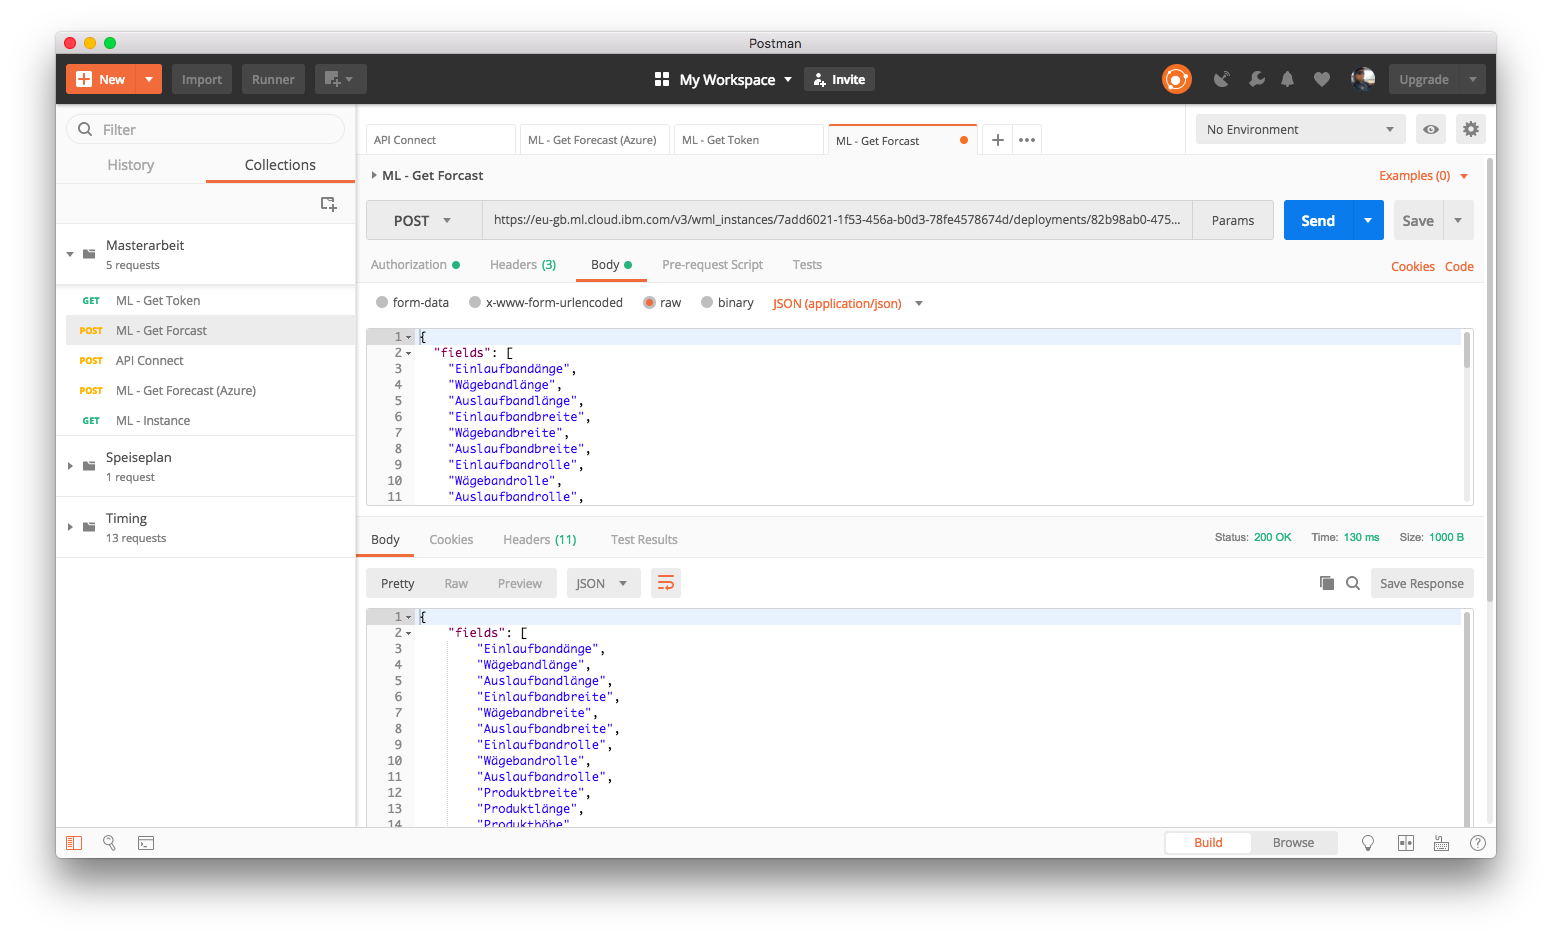
\includegraphics[width=\textwidth]{images/kapitel_3/deployment_postman.png}
    \caption{Beispielrequest von Postman}
    \label{fig:umsetzung_deployment_postman}
\end{figure}

Die Rechte Seite zeigt die Antwort des Web-Service. Dabei werden zu Anfang des JSON-Objektes die Parameter wiederholt,
die an das Interface gesendet wurden. Am Ende sind die vorhergesagten Parameter durch das trainierte Model zu sehen.

Im Eingabe-Parameter \textit{values} muss man ebenfalls die Output-Parameter definieren. Da die Werte keine Rolle
spielen, kann man diese mit den Werten \textit{null} initialisieren. Damit werden sie vom System nicht weiter verwendet.

Auf der Übersichtsseite des REST-Interfaces des
Deployments\footnote{https://watson\-ml\-api.mybluemix.net/?cm\_mc\_uid=61889453441915363064337}, sind noch weitere
Endpunkte und die dafür benötigten Parameter sowie die Rückgabewerte ersichtlich.

\subsection{TensorFlow.js}
Das neuronale Netz ist nun erfolgreich in einem Deployment online zur Verfügung gestellt. Außerdem ist die Funktion
über einen Aufruf mittels Postman überprüft worden. Im Weiteren wird das trainierte Model in eine TensorFlow.js
Applikation eingebaut.

Dies hat nun mehrere Vorteile. Zum einen kann man das trainierte Model unabhängig von einer Cloud-Lösung nutzen. Die
TensorFlow.js Applikation kann zum Beispiel in einen Cloud Foundry-Container geladen werden und ist somit völlig unabhängig
von der Plattform auf der die Applikation läuft. Auch kann sie modular und schnell in beliebigen Regionen instanziiert
werden.

Ein weiterer Vorteil ist die Unabhängigkeit welche damit erreichbar wird. Die Applikation kann selbst verwaltet,
instanziiert oder auch aktualisiert werden.

Natürlich ist es ebenfalls möglich die TensorFlow.js Applikation direkt in die eigene Hauptapplikation zu integrieren
ohne sie als Microservice nutzen zu müssen.

\subsubsection{Model exportieren}
Damit das Model in die TensorFlow.js Applikation eingebunden werden kann, muss es aus dem Watson Studio exportiert werden.
Dies erfolgt über den Modeler Flow.

Da der Entwickler das Model in Kapitel~\ref{subsub:modeler_flow} auf Seite\pageref{subsub:modeler_flow} komplet
eingerichtet und trainiert hat, steht es im Modeler Flow als gelbes Modul bereit.

Über einen Rechtsklick auf das trainierte Model und dem Menüpunkt \texttt{Download Model} kann man das Model auf den
Entwicklungsrechner herunterladen. Bei der Datei handelt es sich um eine pb-Datei. Diese Datei beinhaltet alle wichtigen
Informationen über das gebaute neuronale Netz.

Auf der Seite des
FreeCodeCamps\footnote{https://medium.freecodecamp.org/how-to-deploy-tensorflow-models-to-production-using-tf-serving-4b4b78d41700}
ist eine Beschreibung und der interne Aufbau der gespeicherten Datei ersichtlich. Auch wird dort erklärt, wie die Datei
in andere Anwendungen importiert werden kann.

Im Weiteren kann mit der Entwicklung des Wrappers für das heruntergeladene neuronale Netz begonnen werden. Dafür wird
der Inhalt der Datei in einer TensorFlow.js Applikation importiert und ausgewertet.

\subsubsection{Wrapper entwickeln}
Da das trainierte Model nun offline zur Verfügung steht, kann es im Weiteren mit TensorFlow.js in einem Node.js-Wrapper
genutzt werden.

Die Idee des Wrappers ist es, ein Web-Service zur Verfügung zu stellen, der auf dem Port 80 eine REST-Schnittstelle
beherbergt. Dort findet sich mindestens ein REST-Endpunkt, welcher die Input-Parametern für das trainiert,
neuronale Netz annehmen kann.

Die übergebenen Werte werden anschließend von einer Routine extrahiert und über die TensorFlow.js Bibliothek an das
heruntergeladene neuronale Netz übergeben.

Anschließend übermittelt der Web-Service die durch das neuronale Netz vorhergesagten Parameter zurück an die Applikation,
welche die Anfrage gestellt hat.

Für die Umsetzung des Wrappers sind also zwei Bestandteile elementar. Einerseits muss die Anwendung eine TensorFlow.js
Umgebung schaffen, indem man das heruntergeladene und trainierte Netz einbinden kann. Andererseits muss es eine
REST-Schnittstelle bieten, damit man es von über den API Connect Service ansprechen kann.

Bei der Entwicklung beginnt man am Besten beim REST-Endpunkt, da dieser die Struktur der Anwendung vorgibt. Für die
Implementierung der Endpunkte sind die Libraries \textit{express}\footnote{https://expressjs.com/de},
\textit{body-parser}\footnote{https://github.com/expressjs/body-parser}, \textit{tfjs}\footnote{https://github.com/tensorflow/tfjs} 
und \textit{tfjs-node}\footnote{https://github.com/tensorflow/tfjs-node} sehr hilfreich.

Die \textit{express}-Bibliothek unterstützt bei der Entwicklung eines Web-Servers, welchen man anschließend über den
Port 80 ansprechen kann. Der \textit{body-parser} kümmert sich um das Auslesen der übergebenen Parameter an die
Schnittstelle oder das Bündeln der Rückgabewerte - also um den Umgang mit JSON-Objekten.

Die TensorFlow-Bibliotheken \textit{tfjs} und \textit{tjfs-node} sind für die Verwarbeitung von neuronalen Netzen,
die Übergabe von Parametern an Modelle und das bereitstellen von heruntergeladenen neuronalen Netzen verantwortlich.

Da Node.js und damit der Paketmanager npm schon installiert ist, kann der Entwickler mit \textit{npm init} ein neues 
Projekt starten. Wenn man diesen Befehl in einem noch leeren Ordner ausführt, erscheint eine neue Datei mit dem Namen
\textit{package.json}. In dieser Datei werden unter anderem alle benötigten Abhängigkeiten des Projektes aufgelistet 
um sie später einfach und komfortabel zu installieren.

Hinter den einzelnen Bibliotheken kann man direkt die Version definieren, welche man nutzen möchte. Im Listing ist ein
\textbf{\^}-Symbol vorangestellt. Dies bedeutet, dass die Version, welche heruntergeladen werden soll, zu der angegebenen
Version kompatibel sein muss. Das bedeutet, dass durchaus eine andere Version heruntergeladen werden kann, falls eine
neuere existiert. Allerdings bietet sie mindestens genau die selben Funktionen wie die geforderte.

Auch werden in der Datei der Name, eine Beschreibung und die Version des Projektes angegeben. Außerdem kann man Skripte
definieren, welche man durch kurze Befehle in ein Terminal ausführen kann. Dazu später mehr.

In Listing~\ref{ls:umsetzung_package} auf Seite~\pageref{ls:umsetzung_package} ist die vollständige package.json-Datei
ersichtlich, welche die beiden Bibliotheken als Abhängigkeit entählt und ein paar wenige Parameter wie Name, Beschreibung, 
Version und verwendete Lizenz angibt. 

Auch ist ein script mit dem Namen \textit{start} angegeben. Dies kann später mit dem Befehl \textit{npm start} starten.
Die definition für den Startbefehl kümmert sich anschließend darum, dass intern der Befehl \textit{node server.js}
ausgeführt wird. Diese Datei wird im Weiteren erstellt.

\begin{lstlisting}[language=json, caption=Die komplette package.json, label=ls:umsetzung_package]
{
    "name": "tensorflow_wrapper",
    "version": "1.0.0",
    "description": "A rest-wrapper for a tensorflow net.",
    "main": "server.js",
    "scripts": {
        "start": "node server.js"
    },
    "author": "Lars Helmuth Probst <lars@famprobst.de>",
    "license": "ISC",
    "dependencies": {
        "body-parser": "^1.18.3",
        "express": "^4.16.4",
        "tensorflow/tfjs": "^0.13.2",
        "tensorflow/tfjs-node": "^0.1.19"
    }
}
\end{lstlisting}

Im selben Ordner wie die angelegte package.json kann man nun mittels des Befehls \textit{npm install} alle Abhängigkeiten 
in das Projekt installieren. 

Auch wenn eine selbst benötigte Bibliothek, wie zum Beispiel die express-Library, weitere Abhängigkeiten benötigt, werden 
diese automatisch mitinstalliert. So ist sichergestellt, dass alle geforderten Bibliotheken einwandfrei funktionieren.

Die Ausführung des Befehls hat zur Folge, dass ein neuer Ordner mit dem Namen \textit{node\_modules} erstellt wird. In diesem 
finden sich nun alle geforderten Bibliotheken und deren Abhängigkeiten an einem zentralen Ort und sind zur Verwendung bereit.

Als nächstes kann man mit der Entwicklung des REST-Endpunktes beginnen. Dafür wird eine initiale Datei benötigt, in der der
Express-Server sowie alle REST-Endpunkte definiert sind. 

Diese Datei trägt den Namen \textit{server.js} und ist in Listing~\ref{ls:umsetzung_serverjs} auf 
Seite~\pageref{ls:umsetzung_serverjs} zu sehen. In den ersten drei Zeilen der Datei werden die benötigten Bibliotheken in das 
Programm geladen um sie für andere Routinen verfügbar zu machen. Der Express-Server, der Body-Parser und die 
TensorFlow.js-Runtime ist somit einsatzbereit.

In der fünften Zeile wird in der Variable \textit{app} die Instanz des Express-Servers gespeichert. Somit kann man diesen über
die Variable konfigurieren.

\begin{lstlisting}[language=JavaScript, caption=Die komplette server.js, label=ls:umsetzung_serverjs]
const express = require('express');
const bodyParser = require('body-parser');
const tf = require('@tensorflow/tfjs-node')

const app = express();

app.use(bodyParser.urlencoded({ extended: true }));

app.post('/predict-tensorflow', (req, res) => {
    // TODO TensorFlow.js
    res.send(req.body)
});

app.listen(80, () => {
    console.log('server listening on port 80.');
});
\end{lstlisting}

Die siebte Zeile sorgt dafür, dass man \textit{URL-Encoded}-Daten an den entwickelten REST-Endpunkt schicken kann und man 
diese dann auch verwenden kann. Andernfalls müssten alle Anfragen durch ein API-Gateway gesondert geparst werden.

Durch die Zeile neun bis zwölf wird ein Endpunkt für den Express-Server definiert, welcher in einem weiteren Schritt mit der
TensorFlow.js Logik gefüllt wird. Der Endpunkt bekommt den Namen \textit{predict-tensorflow} und als HTTP-Typ ist \textit{POST}
angegeben. Somit kann man Daten an den Endpunkt schicken.

Mit der Zeile elf werden alle Daten und Informationen, welche an den Endpunkt geschickt werden, auch wieder zurückgegeben. 
Dies dient als ein Test für das richtige Versenden und die richtige Funktion des Endpunktes. Man kann dies zum Beispiel
mit dem Programm Postman verifizieren.

Die letzten drei Zeilen lassen den Express-Server auf Port 80 starten und geben Auskunft darüber, dass der Start des Servers
erfolgreich war. Diese Information wird in der Konsole ausgegeben.

Im Weitern kann man nun die Zeile zehn so erweitern, dass die mitgeschickten Daten auch an das heruntergeladene neuronale
Netz übergeben werden. Das wird durch die Hilfe der TensorFlow.js und der Body-Parser-Bibliothek ermöglicht.

In Listing~\ref{ls:umsetzung_tensorflow} auf Seite~\pageref{ls:umsetzung_tensorflow} sind alle Änderungen für den Einbau des
TensorFlow.js-Wrappers aufgeführt.

\begin{lstlisting}[language=JavaScript, caption=Der TensorFlow.js Programmteil, label=ls:umsetzung_tensorflow]
const mn = new mobilenet.MobileNet(1, 1);
mn.path = "./neural_net.json"
await mn.load()

const predictions = await mn_model.classify(req.body);
res.send(predictions);
\end{lstlisting}

Die Zeilen eins bis drei kümmern sich um das Laden des trainierten Netz von der Festplatte. Dabei ist in der zweiten Zeile
der Name des heruntergeladenen neuronalen Netzes angegeben. Auch einen eventuellen Pfad kann man dort angeben. 

In der fünften Zeile werden die übergebenen Daten des REST-Endpunktes an die TensorFlow.js-Instanz weitergegeben um eine
Vorhersage zu erhalten. Über die letzte Zeile werden die vorhergesagten Parameter wieder zurückgegeben.

Diese Zeilen muss man nun lediglich in die Datei \textit{server.js} in die Zeile elf kopieren, damit die REST-Schnittstelle
vollkommen ist. Die Ursprüngliche elfte Zeile mit der Testrückgabe der gesendeten Parameter muss man dabei entfernen.

Über den Terminal-Befehl \textit{npm start} startet der Express-Server lokal auf dem Entwicklerrechner. Anschließend kann
man mit Postman und dem HTTP-Typ \textit{POST} eine Anfrage an das Erstellte REST-Interface machen um die funktion der 
Anwendung zu überprüfen.

Die entwickelte Applikation soll im Weiteren über eine Domain aus dem Internet aufrufbar sein. Eine Installation in einen
Cloud Foundry-Container, welcher in der IBM Cloud läuft, ist dafür notwendig. Im folgenden Kapitel werden die dafür
nötigen Schritte erläutert.

\subsubsection{Toolchain einrichten}
Die fertig entwickelte Node.js Applikation wird im nächsten Schritt in einen Cloud Foundry-Container installiert. Dies
ermöglicht den Aufruf der Applikation über eine Domain, welche automatisch von der IBM Cloud vergeben wird.

Damit man den geschriebenen Quellcode nicht nach jeder Änderung manuell mittels \texttt{cf push} in einen Cloud
Foundry-Container laden muss, wird hierfür eine Toolchain aus der IBM Cloud genutzt.

Die Nutzung der Toolchain erfordert ein eingerichtetes Git-Repository. Nach jedem \texttt{commit}, welchen man in dieses
Repository schreibt, aktiviert sich die Toolchain selbstständig und lädt den entsprechenden Commit herunter.

Anschließend werden, je nach gewählter und eingerichteter Konfiguration, verschiedene Schritte (Phasen) in der Toolchain
durchlaufen, um die Applikation in einen Cloud Foundry-Container zu installieren.

Dabei ist es möglich die einzelnen Schritte, welche bei einem Deployment durchlaufen werden, selbst zu definieren, oder
eine vorkonfigurierte Toolchain zu nutzen. Es ist allerdings möglich die vorkonfigurierte Toolchain im Nachgang zu
individualisieren. Sie dient lediglich einem schnelleren Start.

Für die Konfiguration der Toolchain muss man die instanziierte Node.js Runtime, in welcher die entwickelte Applikation
laufen soll, in dem IBM Cloud Dashboard auswählen.

Auf der dann folgenden Seite im Tab \texttt{Übersicht} (linke Seite) erscheinen fünf Kacheln mit unterschiedlichen
Informationen. Für die Toolchain ist die Karte mit der Aufschrift \texttt{Continous Delivery} entscheidend. Dort gibt es
einen Button mit der Aufschrift \texttt{Aktivieren}.

Ein Klick auf diesen öffnet die Übersicht und eine visuelle Vorschau der Standardkonfiguration der Toolchain. Nun muss
man einen Name eintragen und die Region auswählen, in der die Toolchain installiert wird. Da die Standardkonfiguration
vorerst völlig ausreichend ist, kann diese direkt übernommen werden. Dafür genügt ein Klick auf \texttt{Erstellen}.

Nach einem kurzen Ladevorgang ist die Toolchain eingerichtet und vorkonfiguriert. Es erscheinen nun vier Karten für
unterschiedliche Bereiche, in denen die IBM Cloud dem Entwicklungszyklus helfen kann.

Im Bereich \texttt{Nachdenken} wird ein Issue-Tracker konfiguriert, in dem zum Beispiel Bugs (Softwarefehler), welche
in der Software entdeckt werden, eingetragen, verwaltet und diskutiert werden können.

In \texttt{Codieren} stehen gleich zwei Kacheln zur Verfügung. Einerseits das konfigurierte Git-Repository, bei dem es
sich um ein auf IBM-Servern gehostetes GitLab handelt. Andererseits findet sich dort eine Web-IDE auf Basis von Eclipse
Orion, mit der der Quellcode der Anwendung online editiert werden kann.

In der letzten Kategorie, \texttt{Bereitstellen}, findet sich die Pipeline, welche im nächsten Schritt näher erläutert
und eingerichtet wird. Mit einem Klick auf die Kachel mit der Aufschrift \texttt{Delivery Pipeline} wechselt man in die
Konfiguration.

Nach dem Laden der Seite erscheinen zwei sogenannte \textit{Phasen} (engl. Stages). Jeder Schritt in der Delivery Pipeline
wird durch eine Phase symbolisiert. In einer Phase können zum Beispiel der Quellcode aus dem Git-Repository geladen, oder
die geschriebenen Tests durchgeführt werden.

Die Standardkonfiguration sieht in der \textit{Build Stage} das Herunterladen des Quellcodes aus dem Git-Repository vor
und in der \textit{Deploy Stage} das Einrichten eines Cloud Foundy-Containers.

Für die Node.js Applikation reicht diese Konfiguration völlig aus, da keine zusätzlichen Installationen oder Einrichtungen
notwendig sind.

In Abbildung~\ref{fig:umsetzung_toolchain_pipeline} auf Seite~\pageref{fig:umsetzung_toolchain_pipeline} ist die
komplette Konfiguration der Toolchain veranschaulicht. Die grünen Balken zeigen einen erfolgreichen Durchlauf einer
einzelnen Phase an.

\begin{figure}[h]
    \centering
    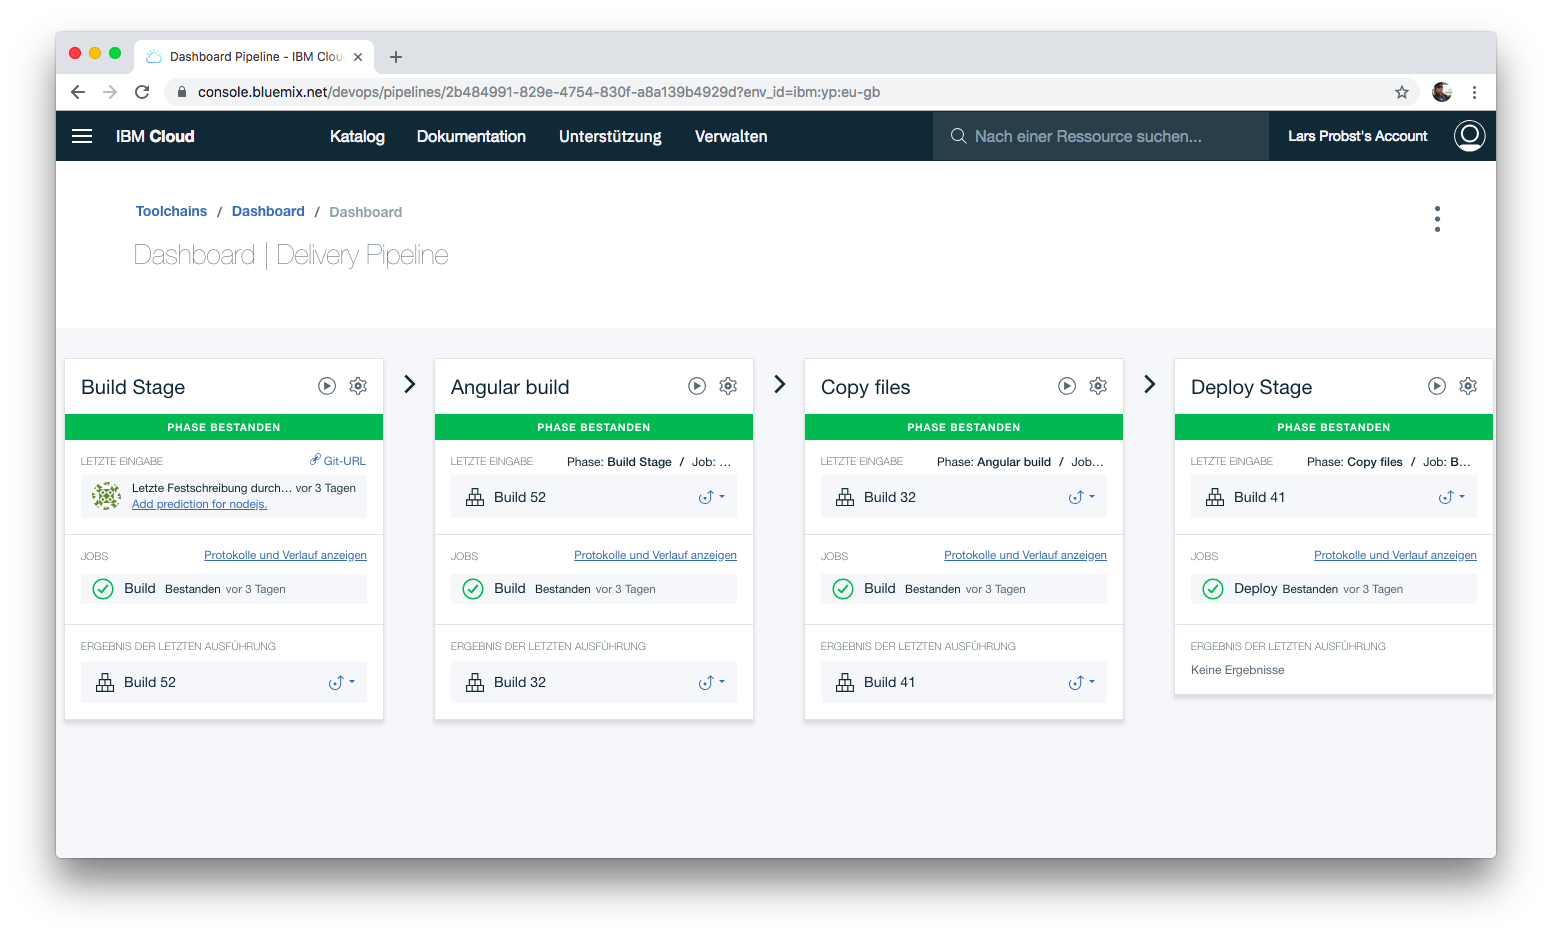
\includegraphics[width=\textwidth]{images/kapitel_3/toolchain_pipeline.png}
    \caption{Übersicht der Toolchain-Konfiguration}
    \label{fig:umsetzung_toolchain_pipeline}
\end{figure}

Als nächstes muss man den geschriebenen Quellcode der Applikation lediglich noch in das, in der Toolchain hinzugefügte,
Git-Repository einchecken. Die URL für das Repository kann man sich in der Toolchain-Übersicht mit einem Klick auf die
Kachel \texttt{Git} anzeigen.

Nach erfolgreichem \texttt{push} der Anwendung in das Git-Repository startet der Deploymentvorgang in der Toolchain
selbstständig. Nach wenigen Minuten ist die Anwendung über ihre URL, welche in der Node.js Runtime definiert ist,
aufrufbar.

Da die Applikation nun im Internet in einem Cloud Foundry-Container zur Verfügung steht, kann diese im nächsten Schritt
mit dem API Connect Service verbunden werden.

Dieser Schritt ist nötig, damit die Schnittstelle der Applikation vom Frontend, welches in Kapitel~\ref{subsec:webseite}
auf Seite~\pageref{subsec:webseite} beschrieben wird, und auch über Postman vereinfacht aufgerufen werden kann.

\subsection{API Connect}
\label{subsec:apiconnect}
Wie in Kapitel~\ref{subsec:Aufruf mit Postman} auf Seite~\pageref{subsec:Aufruf mit Postman} beschrieben, benötigt das
REST-Interface des erstellten Deployments einen Auth-Token. Dieser kann nur über den Aufruf einer anderen
REST-Schnittstelle zur Verfügung gestellt werden.

Damit man diese Schritte vereinfachen kann und das im weiteren Verlauf erstellte Frontend ebenfalls das Deployment aufrufen
kann, werden beide Abfragen in API Connect gebündelt.

Ein weiterer Grund für das Bündeln der beiden Anfragen an den Watson Service ist das Mitschicken des Benutzernamens und
des zugehörigen Passwortes zum generieren des Tokens. Damit diese Daten nicht in der zu entwickelnden Anwendung hinterlegt
werden müssen, kann man diese Zentral in API Connect speichern. Das hat den Vorteil, dass man sie bei Bedarf nur an einer
zentralen Stelle abändern muss.

Desweiteren ist es relativ einfach Daten auszulesen, die von einer Anwendung an die Schnittstelle geschickt werden. Dies
ermöglicht es Angreifern die Daten für andere Zwecke zu missbrauchen.

Ein weiterer Vorteil für die Nutzung von API Connect ist die Bündelung von mehreren Schnittstellen um Vorhersagen zu
beziehen. Aktuell ist es möglich, die Vorhersage aus dem Deployment des Watson Studio Models zu beziehen oder die
entwickelte Node.js Applikation mit TensorFlow.js zu nutzen.

Mittels API Connect kann man die Aufrufe optimal verteilen oder eigene Routen für eine jeweilige Schnittstelle bauen.
Außerdem kann man Änderungen schnell und kompfortabel in einem Online-Editor anpassen.

Die anpassung der Routen in API Connect bedürfen keinerlei Programmierkenntnisse uns sind sehr schnell umgesetzt und in
Echtzeit veröffentlich.

\subsubsection{API Connect einrichten}
Der in Kapitel~\ref{subsec:vorbereitung_apiconnect} auf Seite~\pageref{subsec:vorbereitung_apiconnect} instanziierte
Service wird im folgenden konfiguriert und eingerichtet. Dazu muss man ihn aus dem IBM Cloud Dashboard heraus aufrufen.
Nach dem Klick auf den Service-Namen erscheint eine Seite mit hilfreichen Informationen zum Service.

Über die Schaltfläche \texttt{Open API Connect} gelangt man auf das API Connect Dashboard. In diesem muss man zuerst ein
automatisch angelegten Katalog benennen. In diesem Katalog werden alle Informationen zur API gespeichert.

Veröffentlichte APIs werden automatisch in diesem Katalog aufgelistet. Nach der fertigen Einrichtung des Kataloges gelangt
man über einen Klick auf \texttt{Entwürfe} auf die Entwurfsübersicht.

In dieser muss man den Menüpunkt \texttt{APIs} auswählen. In der erscheinenden Liste werden alle APIs, welche im Weiteren
erstellt werden, aufgelistet. Aktuell existieren hier aber noch keine. Dies kann der Nutzer über den Button
\texttt{Hinzufügen} und dann \texttt{Neue API} ändern.

Nachdem man den Titel, einen Namen und eine beliebige Version hinterlegt hat, kann man die API mit \texttt{API erstellen}
in die Liste aufnehmen. Sie erscheint nun mit dem definierten Namen. Über einen Klick auf diesen lässt sich die
Konfiguration der API öffnen.

Für die Konfiguration einer API existieren drei wichtige Untermenüs. In \texttt{Gestalten} lassen sich Name, Beschreibung,
Version, die Sicherheitsdefinitionen sowie die zur Verfügung gestellten Pfade und dafür vorgesehene Parameter definieren.

Der Menüpunkt \texttt{Quelle} zeigt die komplette Konfiguration der API in Swagger-Notation an. Hier getätigte Änderungen
werden automatisch in den anderen beiden Menüpunkten übernommen.

Im letzten Menüpunkt, \texttt{Assemblieren}, kann man die Funktionen der API definieren. Dazu zählen zum Beispiel die
einzelnen Schritte, welche bei einem Endpunkt durchlaufen werden müssen. Hier wird der Inhalt der API definiert.

Um mit der Konfiguration zu starten, muss der Nutzer zuallererst die einzelnen Pfade, welche zur Verfügung stehen sollen,
definieren. Dazu wird in den Menüpunkt \texttt{Gestalten} gewechselt und im linken Menü dann in \texttt{Pfade}.

Über das kleine Plus-Zeichen im rechten Bereich kann der Nutzer einen neuen Pfad hinzufügen. Pfade sind die Endpunkte
einer REST-Schnittstelle. Jede URL ist ein Endpunkt. Über jeden einzelnen Endpunkt können verschiedene HTTP-Requests
angesteuert werden. Die häufigsten sind \textit{GET}, \textit{POST}, \textit{PUT} und \textit{DELETE}.

Direkt nach einem Klick auf das Plus-Zeichen erscheint ein neuer Pfad mit dem Namen \textit{/pfad-1}. Diesen kann man
durch einen Klick aufklappen. Es erscheinen nun die Konfigurationsparameter für den Endpunkt. Als \textit{Pfad} wird nun
ein Name vergeben, über den das Watson Studio Deployment aufgerufen werden kann. Ein Beispiel hierfür ist
\textit{predict-watson}.

Da in der jetzigen Version für die Parameter keine Validierung vorgenommen wird, kann die Einstellung dieser ignoriert
werden. Allerdings muss man nun eine neue Operation hinzufügen. Dabei handelt es sich um die HTTP-Typen. Da von der
späteren Anwendung Daten an die Schnittstelle geschickt werden sollen, muss es eine Operation vom Typ \textit{POST} sein.

Über den Button \texttt{Operation hinzufügen} kann man diese hinzufügen. In dem Dropdown-Menü muss der Nutzer dann den
entsprechenden \texttt{POST}-Eintrag auswählen. Dieser erscheint sogleich in der Liste und wird grün hinterlegt.

Mit einem Klick auf den \textit{POST}-Eintrag wechselt man in die weitere Konfiguration. Die weitere Konfiguration ist
für die Schnittstelle uninteressant und kann wieder geschlossen werden.

Diese Schritte muss man nun auch für einen weiteren Pfad mit dem Namen \textit{predict-tensorflow} durchführen. Diese
Route ist für die Kommunikation mit der Node.js Applikation notwendig. Sie erhält ebenfalls eine Operation vom Typ
\textit{POST}.

Somit sind erfolgreich zwei Endpunkte mit den Namen \textit{predict-watson} und \textit{predict-tensorflow} angelegt
worden. Diese haben jeweils eine Operation vom Typ \textit{POST}.

Als weitere wichtige Einstellung muss man unter \texttt{Lebenszyklus} den Schalter bei \texttt{CORS} aktivieren und da
im ersten Schritt mit keiner Sicherheit gearbeitet wird, kann der entsprechende Menüpunkt übersprungen werden.

Über das Disketten-Symbol am oberen rechten Rand kann man die aktuelle Einstellung zur Sicherheit speichern. Eine
entsprechende Meldung quittiert die Speicherung.

Die Grundeinstellungen der Schnittstelle sind somit getätigt. Im Weiteren muss der Entwickler die API über
\texttt{Assemblieren} mit dem richtigen Verhalten versehen. Dazu wechselt man über den entsprechenden Menüpunkt in einen
fast leeren Arbeitsbereich.

Hier finden sich im linken Bereich alle möglichen Bausteine um die API mit Funktionen und intelligenz zu füllen. Im
mittleren Teil, dem Arbeitsbereich, ist lediglich ein Punkt hinterlegt. Dieser dient als Einstieg bei einem Aufruf der
Schnittstelle. Ein Aufruf der API landet immer in diesem Knoten und kann dann verteilt werden.

Als einer der ersten Schritte soll die Schnittstelle selbstständig einen Auth-Token vom Watson Studio abgreifen. Dazu
wird das Modul \texttt{Aufrufen} benötigt. Mittels Drag \& Drop kann man dieses Modul in den Arbeitsbereich, direkt
hinter den schon hinterlegten Punkt setzen. Automatisch werden die beiden Module verbunden.

Durch ein doppelten Klick auf das Modul öffnet sich die entsprechende Konfiguration am rechten Bildschirmrand. Als Titel
kann man zum Beispiel \enquote{Get Token} definieren. Als URL dient die Schnittstelle des Watson Studios, welche mit
\enquote{https://eu-gb.ml.cloud.ibm.com/v3/identity/token} angegeben ist.

Der Benutzername und das zugehörige Passwort sind im instanziierten Watson Studio Service zu sehen. Man gelangt über das
IBM Cloud Dashbaord auf die Seite.

Als \textit{HTTP-Methode} muss \texttt{GET} ausgewählt sein. In der Schnittstelle des Watson Studios, existiert auf
diesem Endpunkt lediglich diese Operation.

Als letzte Einstellung muss man als \textit{Antwortobjektvariable} die Bezeichnung \enquote{newtoken} eintragen. Die
Konfiguration des Modules ist damit abgeschlossen und es kann mit den nächsten Modulen fortgefahren werden.

Da die Schnittstelle des Watson Studios den Auth-Token als Rückgabeparameter besitzt, muss man diesen in API Connect
speichern und allgemein zur Verfügung stellen. Dies kann nur über das Modul \texttt{Zuordnen} erfolgen.

Dieses Modul kann man der Kategorie \textit{Umwandlungen} entnehmen und es direkt nach dem Request-Modul platzieren. Es
reiht sich somit dahinter ein. Ein doppelter Klick öffnet die Konfiguration des Modules. Da hier nur ein Parameter
gespeichert werden muss, ist die Konfiguration recht simpel.

In der Spalte Eingabe kann man über den Stift einen neuen Eintrag hinzufügen. Als Kontextvariable ist
\enquote{newtoken.body.token} zu definieren. Dabei handelt es sich um den Rückgabeparameter des vorangestellten
Request-Modules und das JSON-Objekt \enquote{token}, welches von der Schnittstelle zurückgegeben wird.

Als Name der Variable wird \enquote{Token Input} definiert, der Inhaltstyp ist \enquote{text/plain} und die Definition
ist \enquote{string}. Über \texttt{Fertig} kann man die Konfiguration speichern.

Nun muss in der Spalte Ausgabe eine interne Variable definiert werden, welche den Auth-Token speichert. Dafür wird über
den Stift ein neuer Eintrag angelegt. Die Kontextvariable ist \enquote{newtoken} und der Name \enquote{Token Output}.
Als Inhaltstyp wird \enquote{text/plain} ausgewählt, da die Variable auf der Seite der Eingabe als Text definiert ist.
Somit wird auch die Definition auf \enquote{string} gesetzt.

Nachdem auf beiden Seiten nun ein Eintrag erscheint, muss man diese beiden über die rundlichen Punkte verbinden. Eine
grüne Linie symbolisiert anschließend die Verbindung. Die Konfiguration der Zuordnung ist damit fertiggestellt.

Da bei der Schnittstelle mir CORS gearbeitet wird, muss man in einem nächsten Schritt den Header setzen, welche Anfragen
erlaubt sind. Dafür verwendet man einen \textit{Gateway Script}. Dies platziert man einfach hinter dem Zuordnungs-Modul.

Die Konfiguration des Moduls entspricht Quellcode in JavaScript. Die Zeilen in Listing~\ref{ls:umsetzung_cors} auf
Seite~\pageref{ls:umsetzung_cors} definieren die entsprechenden Einstellungen.

\begin{lstlisting}[language=JavaScript, caption=Gateway Script für CORS, label=ls:umsetzung_cors]
// Set CORS headers
apim.setvariable('message.headers.Access-Control-Allow-Origin', '*')
apim.setvariable('message.headers.Access-Control-Allow-Headers', 'Origin, X-Requested-With, Content-Type, Accept')
\end{lstlisting}

Die zweite Zeile besagt, dass die nachfolgende Konfiguration für \textit{alle} Requests zählt, die diese Schnittstelle
aufrufen. Die dritte Zeile besagt, dass die Anfragen akzeptiert werden sollen. Somit kann jede Anwendung mit dieser
Schnittstelle kommunizieren.

Bei einer späteren Konfiguration könnte man Anwendungen, welche auf die Schnittstelle zugreifen können, hier
einschränken. Dazu muss man die IP der Anwendung kennen, welche mit der Schnittstelle kommunizieren möchte. Diese kann
man dann in die zweite Zeile eintragen (das \enquote{*} ersetzen).

Da es zwei Endpunkte für die Schnittstelle geben wird, braucht man nun einen \textit{Operationsswitch}, um je nach
gefordertem Endpunkt auch die richtigen Informationen zurückgeben zu können.

Dieser Switch wird direkt nach dem Gateway Script angeordnet. In der Konfiguration des Switches kann der Nutzer über den
Button \texttt{+ Pfad} einen neuen Zweig hinzufügen. Insgesamt werden zwei Stück benötigt. Der erste Fall ist für
\textit{predict-watson} da. Der Zweite für \textit{predict-tensorflow}.

\subsubsection*{Pfad für das Watson Deployment}
Für den Pfad des \textit{predict-watson} wird ein weiteres Gateway Script benötigt, welches den Header für die Anfrage
an des Watson Studio Deployment setzt. Für die Einstellungen sind die JavaScript Zeilen in
Listing~\ref{ls:umsetzung_settoken} auf Seite~\pageref{ls:umsetzung_settoken} zuständig.

\begin{lstlisting}[language=JavaScript, caption=Gateway Script für den Authorization-Token, label=ls:umsetzung_settoken]
// Set the token
var token = apim.getvariable('newtoken');
apim.setvariable('message.headers.authorization', 'Bearer' + token);
\end{lstlisting}

In der zweiten Zeile wird der Token, welcher in dem Modul \textit{Zuordnung} gespeichert wurde, ausgelesen. Die dritte
Zeile sorgt dafür, dass ein Header mit dem Key \textit{authorization} und dem Value \textit{Bearer + token} gesetzt wird.

Diese Einstellungen sind wichtig, damit der spätere Request an das Watson Studio Deployment die richtigen Benutzerdaten
erhält um die Anfrage für gültig zu erklären.

Ein weiteres Gateway Script sorgt dafür, dass die ursprünglich übergebenen Parameter an den API Connect Service (mit den
Input-Werten für die Vorhersage) auch an den nächsten Request weitergegeben werden können.

Dafür setzt man die alten Werte als neue Message-Werte. Das Listing~\ref{ls:umsetzung_header} auf
Seite~\pageref{ls:umsetzung_header} veranschaulicht das vorgehen.

\begin{lstlisting}[language=JavaScript, caption=Gateway Script zum Setzen des Message-Bodys, label=ls:umsetzung_header]
// Get variables
var request = apim.getvariable('request.body');
apim.setvariable('message.body', request);
\end{lstlisting}

Im letzten Schritt muss man ein weiteres Aufruf-Modul hinzufügen. Dies erledigt den eigentlichen Aufruf an das Watson
Studio Deployment. Dazu wird das Modul als das Nächste in die Reihe eingefügt. In der Konfiguration muss man lediglich
die URL des Deployments hinzufügen. Diese ist auf der Seite des Deployments ersichtlich.

Damit ist dieser Pfad fertig konfiguriert und kann mit einem Aufruf verifiziert werden. Im nächsten Schritt wird der
zweite Pfad eingerichtet.

\subsubsection*{Pfad für den TensorFlow Container}
Die Einrichtung des TensorFlow-Pfades ist sehr ähnlich zum vorherigen Pfad. Allerdings bedarf es keines Gateway Scriptes
zum setzen eines Authorization Tokens, da dieser hier nicht benötigt wird. Die anderen Module kann man kopieren und in
dem Pfad einsetzen. Lediglich das Aufrufen-Modul benötigt weitere Konfiguration.

In diesem muss nicht die URL des Watson Studio Deployments definiert sein, sondern man muss die des Cloud
Foundry-Containers einsetzen. Anschließend sollte man die Konfiguration über das Disketten-Symbol speichern.

Die Konfiguration des API Conenct Services ist somit abgeschlossen und man kann diese im eingerichteten Katalog
veröffentlichen.

\subsubsection{API Veröffentlichen}
In der Abbildung~\ref{fig:umsetzung_api_connect} auf Seite~\pageref{fig:umsetzung_api_connect} ist der fertig eingerichtete
API Connect Flow dargestellt. Dieser umfasst alle notwendigen Module und Einstellungen.

\begin{figure}[h]
    \centering
    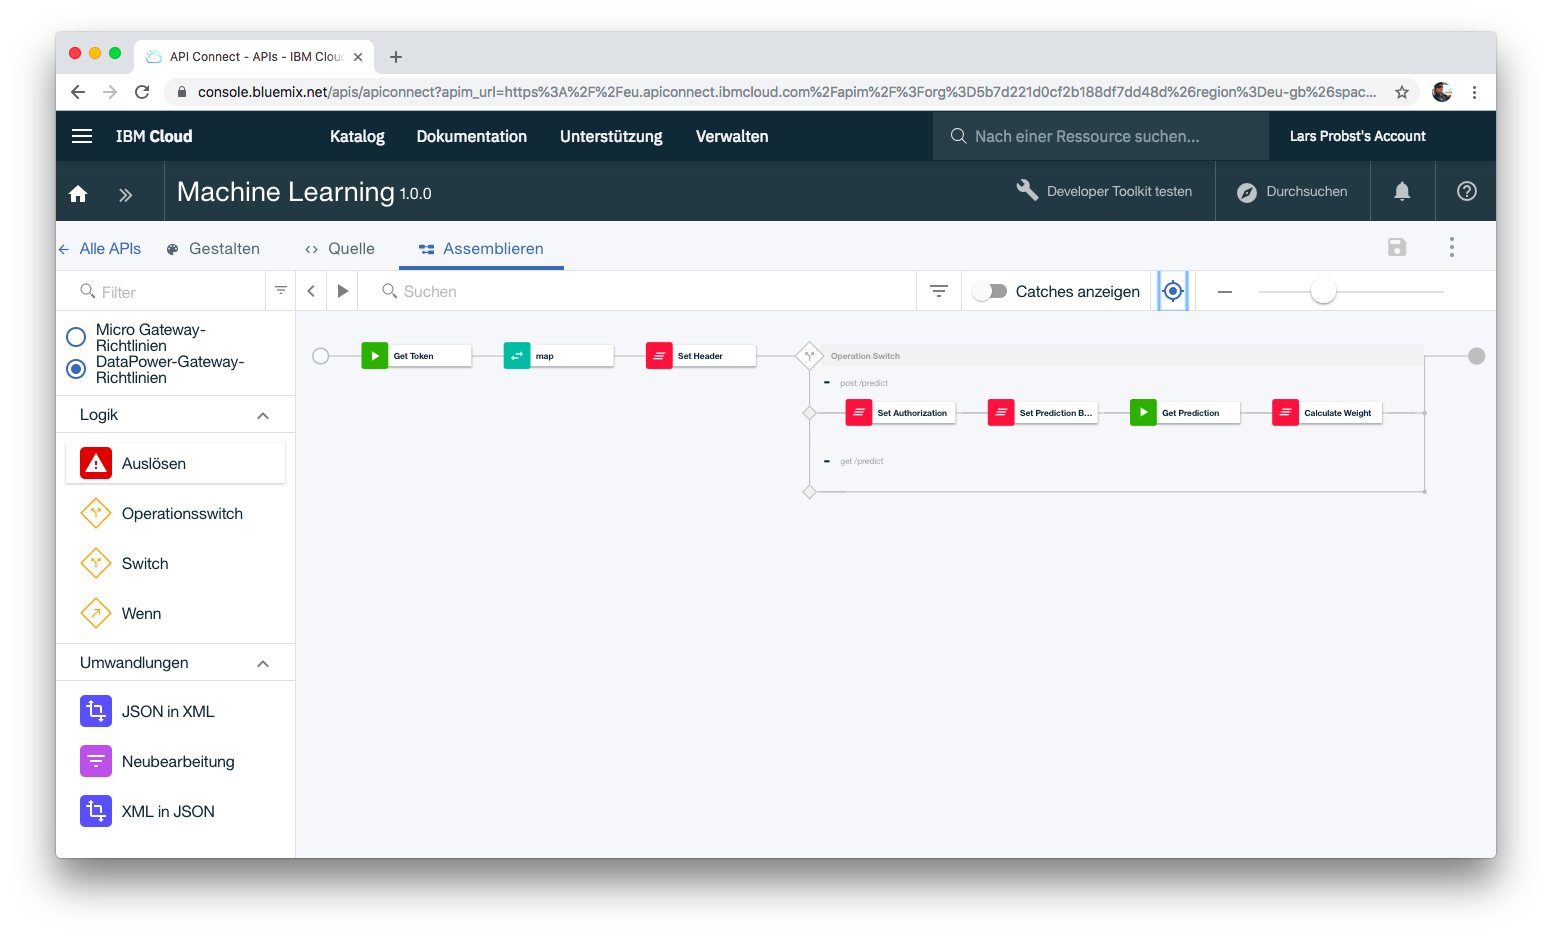
\includegraphics[width=\textwidth]{images/kapitel_3/api_connect.png}
    \caption{Kompletter API Connect Flow}
    \label{fig:umsetzung_api_connect}
\end{figure}

Über den Play-Button am linken oberen Rand, kann man die aktuelle Konfiguration des API Connect Services bauen lassen.
Als Katalog sollte man den anfangs angelegten Katalog definieren. Im Bereich Produkt muss der Nutzer ein Neues anlegen.

Bei dem Produkt handelt es sich um einen Namen für den Service. Die API läuft später unter diesem Produkt-Namen und kann
in dem anfangs erstellten Katalog über das Produkt gefunden werden.

So ist es möglich mehrere APIs für einen Produkt zu definieren. Ein Endnutzer kann sich ein Produkt dann über den Katalog
beziehen und die angelegte API nutzen.

Nun kann man mit \texttt{Produkt veröffentlichen} dieses veröffentlichen und nutzbar machen. Dieser Vorgang kann bis zu
wenigen Minuten dauern.

\subsubsection{API durchsuchen}
Auf dem API Connect Dashboard kann der Benutzer über die rechts oben angelegte Schaltfläche \texttt{Durchsuchen} auf ein
Untermenü zugreifen. In diesem werden alle Kataloge und Entwürfe aufgelistet, die durch ihn erstellt wurden.

Mit einem Klick auf den ersten Eintrag in der Kategorie \textit{Katalog} gelangt man auf eine Übersicht aller
API-Endpunkte, welche sich in diesem Katalog befinden.

Aktuell sollten im linken Feld lediglich zwei Endpunkte zu sehen sein. Der Endpunkt \textit{predict-watson} für das
Watson-Deployment und der Endpunkt \textit{predict-tensorflow} für den Node.js Wrapper. Auch sollten beide über
den HTTP-Type \textit{POST} definiert sein.

Außerdem könnte in diesem Bereich nach einem Endpunkt gesucht oder die Endpunkte sortiert werden. Jeder Eintrag in der Liste
kann angeklickt werden. Daraufhin wird die mittlere Ansicht, in der Informationen zum Endpunkt stehen, zu der jeweiligen
Stelle gescrollt.

Auch kann man der mittleren Spalte für jeden Endpunkt Informationen zu den verwendeten und produzierten Datentypen
entnehmen. Diese Informationen können bei der Konfiguration des API-Endpunktes angegeben werden. Dies ist in
Kapitel~\ref{subsec:apiconnect} auf Seite~\pageref{subsec:apiconnect} erklärt.

Jede zusätzliche Information, die bei der Konfiguration eingetragen wird, erweitert die Ansicht des mittleren Bereiches
um die jeweilige Informationen.

Im rechten Bereich der Ansicht werden Beispielaufrufe angezeigt, wie man die jeweiligen Endpunkte zum Beispiel mit dem
Befehlsprogramm \textit{curl} aufrufen kann. Dies ist hilfreich um die Endpunkte zu testen oder in Erfahrung zu bringen,
wie die Rückgabewerte aussehen.

Außerdem kann man sich die Aufrufe mit anderen Programmiersprachen anschauen. Dies erleichtert die Entwicklung und
Einbindung der Schnittstelle in eigene Programme erheblich.

Als letzte Funktion kann man im rechten Bereich die API-Endpunkte auch direkt online testen. Dies ist hilfreich um die
Funktion des Endpunktes zu überprüfen ohne ein externes Tool nutzen zu müssen.

Bei der Ansicht handelt es sich um eine Darstellung der automatisch generierten Konfigurationsdatei (\textit{yaml}-Datei)
mit einer Swagger-UI\footnote{https://swagger.io/tools/swagger-ui}, welche von IBM optisch angepasst wurde.

\subsubsection{Developer Toolkit}
Ebenfalls über das API Connect Dashboard kann der Entwickler auf den Menüpunkt \texttt{Developer Toolkit} zugreifen.
Dieser zeigt eine Anleitung, wie man die erstellte API auf einem eigenen Server einrichten kann. Dafür sind lediglich
drei einfache Schritte notwendig.

Zuallererst muss man das Programm \textit{API Connect} mittels npm herunterladen und installieren. Anschließens wird über
die Funktion \textit{loopback} eine neue API auf dem lokalen API Connect Service eingerichtet. Der Wizzard führt einen
durch die benötigte Konfiguration.

Nun kann man die Web-Oberfläche des lokalen API Connect starten und seine erstellte, noch leere API, sehen. Anschließend
muss man nur noch die Konfigurations-Datei der online erstellten API kopieren und in den lokalen Service einfügen.

Über den Menüpunkt \texttt{Run Your API}, gelangt man auf eine weitere Anleitung, welche das starten und zur Verfügung
stellen der lokal erstellten API erläutert.

Im letzten Schritt, welchen man über die Schaltfläche \texttt{Publish Your API to IBM Cloud} erreicht, wird Schritt für
Schritt erklärt, wie man die lokal erstellte API nun wieder in der IBM Cloud im Service Watson Studio verfügbar machen
kann.

Dies ist dann sinnvoll, wenn man lokal Änderungen vorgenommen hat und diese wieder online einspielen möchte.

Nach einem Neustart des lokalen Services kann die API genutzt werden und man ist nicht mehr auf eine Cloud-Lösung
angewiesen.

Dies kann diverse Vorteile für die Erstellung einer eigenen Architektur haben. Gerade wenn Applikationen lediglich im
internen Netz zur Verfügung stehen, man allerdings den API Connect Service nutzen möchte.

Oder zum offline Erstellen einer API, da bei der Entwicklung nicht immer eine Verbindung zu den IBM Servern gewährleistet
werden kann.

Eine detailliertere Anleitung steht auf der geöffneten Webseite zur Verfügung. Dort kann man sich die einzelnen Befehle
und Kommandos direkt herauskopieren um diese ausführen.